\chapter{Logika rozmyta i zbiory rozmyte}\label{ch:lst-fuzzy-logic}

\section{Wielowartościowość i zbiory rozmyte}
Stopień prawdziwości zdania nie jest prawdopodobieństwem zdarzenia.
W logice rozmytej interpretacje spójników zależą od wybranego systemu,
a nie tylko od zbioru wartości $[0,1]$.
\begin{definicja}\label{def:lst-fuzzy-set}
Zbiór rozmyty $A$ w $X$ jest funkcją przynależności $\mu_A:X\to[0,1]$.
Klasyczne podzbiory odpowiadają funkcjom charakterystycznym $\chi_E$.
Porządek zawierania określa nierówność punktowa funkcji przynależności.
Jądro to $\{x:\mu_A(x)=1\}$, nośnik to $\{x:\mu_A(x)>0\}$, a
przekrój na poziomie $\alpha\in(0,1]$ to $A_\alpha=\{x:\mu_A(x)\geq\alpha\}$.
\end{definicja}
\begin{twierdzenie}\label{thm:lst-fuzzy-cuts}
Przekroje wyznaczają zbiór rozmyty:
\[
\mu_A(x)=\sup(\{0\}\cup\{\alpha\in(0,1]:x\in A_\alpha\}).
\]
Ponadto dla $0<\alpha\leq\beta\leq1$ mamy $A_\beta\subseteq A_\alpha$,
a $A_\alpha=\bigcap_{0<\beta<\alpha}A_\beta$.
\end{twierdzenie}
\begin{proof}
Dodatnie poziomy zawierające $x$ tworzą przedział $(0,\mu_A(x)]$,
pusty gdy $\mu_A(x)=0$. Stąd pierwszy wzór i monotoniczność.
Jeśli $\mu_A(x)<\alpha$, istnieje $\beta$ między $\mu_A(x)$ a $\alpha$,
więc $x$ nie należy do przecięcia. Druga inkluzja wynika z monotoniczności.
\end{proof}
\begin{twierdzenie}[Charakteryzacja rodzin przekrojów]
\label{thm:ncl-cut-characterization}
Niech $(C_\alpha)_{\alpha\in(0,1]}$ będzie rodziną podzbiorów
zbioru $X$. Istnieje dokładnie jeden zbiór rozmyty $A$ w $X$
taki, że $A_\alpha=C_\alpha$ dla każdego $\alpha\in(0,1]$,
wtedy i tylko wtedy, gdy
\[
  C_\beta\subseteq C_\alpha\quad(0<\alpha\leq\beta\leq1),
  \qquad
  C_\alpha=\bigcap_{0<\beta<\alpha} C_\beta
  \quad(0<\alpha\leq1).
\]
\end{twierdzenie}
\begin{proof}
Konieczność warunków oraz jednoznaczność wynikają z
Twierdzenia~\ref{thm:lst-fuzzy-cuts}. Dla dostateczności
przyjmijmy
\[
 \mu(x)=\sup\bigl(\{0\}\cup\{\alpha\in(0,1]:x\in C_\alpha\}\bigr).
\]
Jeżeli $x\in C_\alpha$, to $\mu(x)\geq\alpha$ z definicji
supremum. Odwrotnie, niech $\mu(x)\geq\alpha>0$.
Dla każdego $\beta\in(0,\alpha)$ istnieje $\gamma>\beta$
takie, że $x\in C_\gamma$: w przeciwnym razie $\beta$
byłoby ograniczeniem górnym zbioru pod supremum.
Z monotoniczności $x\in C_\beta$. Drugi warunek daje
$x\in C_\alpha$. Zatem $\{x:\mu(x)\geq\alpha\}=C_\alpha$.
\end{proof}

\begin{przyklad}[Malejąca rodzina nie wystarcza]
\label{ex:ncl-cut-discontinuity}
Niech $X=\{x\}$ oraz $C_\alpha=X$ dla $0<\alpha<1/2$
i $C_\alpha=\varnothing$ dla $1/2\leq\alpha\leq1$.
Rodzina jest malejąca, lecz
\[
 C_{1/2}=\varnothing\ne X=\bigcap_{0<\beta<1/2}C_\beta.
\]
Gdyby były to słabe przekroje pewnej funkcji przynależności,
wzór rekonstrukcji dawałby $\mu(x)=1/2$. Wówczas jednak
$x$ należałby do przekroju na poziomie $1/2$. Rodzina ta
jest natomiast rodziną przekrojów ścisłych
$\{x:\mu(x)>\alpha\}$ funkcji stale równej $1/2$.
\end{przyklad}

\begin{uwaga}[Poziom zerowy i nośnik]\label{rem:ncl-zero-cut}
Słaby przekrój na poziomie $0$ jest całym $X$, niezależnie
od funkcji przynależności. Nośnik w przyjętym tu znaczeniu
jest przekrojem ścisłym na poziomie $0$:
\[
 \{x:\mu_A(x)>0\}=\bigcup_{n=1}^\infty A_{1/n}.
\]
Inkluzja od prawej do lewej wynika z $1/n>0$; dla
$\mu_A(x)>0$ istnieje $n\geq1$ takie, że $1/n\leq\mu_A(x)$,
co daje drugą inkluzję. Jeżeli $X$ jest przestrzenią
topologiczną, należy odróżnić ten zbiór od jego domknięcia,
nazywanego niekiedy nośnikiem topologicznym. W szczególności
dla liczb rozmytych końce domknięcia nośnika mogą mieć
stopień przynależności równy zero.
\end{uwaga}

\begin{przyklad}[Trójkątna funkcja przynależności]
Dla $a<b<c$ połóżmy
\[
\mu(x)=\max\left(0,\min\left(\frac{x-a}{b-a},\frac{c-x}{c-b}\right)\right).
\]
Rozwiązanie obu nierówności liniowych daje
$A_\alpha=[a+\alpha(b-a),c-\alpha(c-b)]$.
\begin{center}
\begin{tikzpicture}[x=1.1cm,y=2.6cm,>=Stealth]
\draw[->] (0,0)--(6,0) node[right]{$x$};
\draw[->] (0,0)--(0,1.15) node[above]{$\mu(x)$};
\fill[blue!12] (1,0)--(3,1)--(5,0)--cycle;
\draw[thick,blue!70!black] (0,0)--(1,0)--(3,1)--(5,0)--(6,0);
\draw[dashed] (0,0.5) node[left]{$\alpha$}--(4,0.5)--(4,0);
\draw[dashed] (2,0.5)--(2,0);
\draw[very thick,teal!70!black] (2,0)--(4,0) node[midway,below=5pt]{$A_\alpha$};
\draw (0,1) node[left]{$1$};
\end{tikzpicture}
\end{center}
\end{przyklad}
\section{Normy trójkątne i konormy}
Kres dolny i górny w porządku punktowym to minimum i maksimum.
Ich przekroje są odpowiednio przecięciem i sumą przekrojów.
\begin{definicja}\label{def:lst-fuzzy-tnorm}
Norma trójkątna $T:[0,1]^2\to[0,1]$ jest przemienna,
łączna, niemalejąca w obu argumentach i spełnia $T(a,1)=a$.
\end{definicja}
\begin{lemat}\label{lem:lst-fuzzy-tnorm-bound}
$T(a,0)=0$ oraz $T(a,b)\leq\min(a,b)$.
\end{lemat}
\begin{proof}
$0\leq T(a,0)\leq T(1,0)=0$ i $T(a,b)\leq T(a,1)=a$;
przemienność daje ograniczenie przez $b$.
\end{proof}
\begin{przyklad}\label{ex:lst-fuzzy-three-tnorms}
Trzy ciągłe normy trójkątne to
\[
T_G(a,b)=\min(a,b),\quad T_P(a,b)=ab,\quad
T_L(a,b)=\max(0,a+b-1).
\]
Dla minimum i iloczynu aksjomaty wynikają z własności porządku
i mnożenia. Dla $T_L$ łączność wynika z równości obu sposobów
złożenia do $\max(0,a+b+c-2)$; pozostałe aksjomaty wynikają wprost
ze wzoru. Dla $a=b=0{,}7$ wartości wynoszą $0{,}7$, $0{,}49$, $0{,}4$.
\end{przyklad}
\begin{definicja}[Konorma trójkątna]\label{def:ncl-tconorm}
Konorma trójkątna $S:[0,1]^2\to[0,1]$ jest przemienna,
łączna, niemalejąca w obu argumentach i spełnia $S(a,0)=a$.
\end{definicja}
Konorma dualna względem negacji $N(a)=1-a$ ma postać
$S(a,b)=1-T(1-a,1-b)$. Przemienność i łączność wynikają z
przemienności i łączności $T$, monotoniczność z dwukrotnego
odwrócenia porządku, a $S(a,0)=a$ z elementu neutralnego $T$.
Definicja daje $N(S(a,b))=T(N(a),N(b))$, a inwolucja $N$
daje drugie prawo de Morgana.

\begin{stwierdzenie}[Minimum i idempotentność]\label{prop:ncl-tnorm-idempotence}
Norma trójkątna $T$ spełnia $T(a,a)=a$ dla każdego
$a\in[0,1]$ wtedy i tylko wtedy, gdy $T(a,b)=\min(a,b)$.
\end{stwierdzenie}
\begin{proof}
Dla $a\leq b$ monotoniczność i Lemat~\ref{lem:lst-fuzzy-tnorm-bound}
dają $a=T(a,a)\leq T(a,b)\leq a$. Przypadek $b\leq a$
wynika z przemienności. Odwrotny kierunek jest bezpośredni.
\end{proof}
W szczególności nie każda koniunkcja rozmyta odpowiada
przecięciu w sensie przekrojów. Dla $a=b=3/4$ norma
Łukasiewicza daje $T_L(a,b)=1/2$, więc na poziomie
$\alpha=3/4$ oba argumenty przekraczają próg lub są mu
równe, natomiast wynik koniunkcji nie osiąga progu.

\begin{definicja}[Ciągłość normy trójkątnej]\label{def:ncl-left-continuity}
Normę $T$ nazywamy lewostronnie ciągłą, jeżeli dla każdego
$a\in[0,1]$ i każdego niemalejącego ciągu $(c_n)$ z granicą
$c\in[0,1]$ zachodzi
$T(a,c_n)\to T(a,c)$. Przez przemienność analogiczny
warunek zachodzi w pierwszym argumencie. Ciągłość
w zwykłym sensie oznacza ciągłość funkcji dwóch zmiennych
na $[0,1]^2$ i pociąga lewostronną ciągłość.
\end{definicja}

\begin{przyklad}[Minimum nilpotentne]\label{ex:ncl-nilpotent-minimum}
Norma trójkątna
\[
 T_{\mathrm{NM}}(a,b)=
 \begin{cases}
 0,&a+b\leq1,\\
 \min(a,b),&a+b>1
 \end{cases}
\]
jest lewostronnie ciągła, lecz nie jest ciągła.
Przemienność, monotoniczność i neutralność jedynki wynikają
ze wzoru. Dla trzech liczb $x\leq y\leq z$ wszystkie trzy
sposoby wyboru pierwszej pary do mnożenia dają $x$,
gdy $x+y>1$. Gdy $x+y\leq1$, mnożenie najpierw pary
$(x,y)$ daje zero; para $(y,z)$ daje zero lub $y$, a para
$(x,z)$ daje zero lub $x$, więc po pomnożeniu przez trzeci
czynnik wynik również jest zerem. Dowodzi to łączności.
Dla ustalonego $a$ funkcja $b\mapsto T_{\mathrm{NM}}(a,b)$
jest zerowa do punktu $1-a$ włącznie, a powyżej niego
równa minimum. Jest zatem lewostronnie ciągła.
Jednak $T_{\mathrm{NM}}(1/2,1/2)=0$, podczas gdy dla
$b>1/2$ mamy $T_{\mathrm{NM}}(1/2,b)=1/2$.
\end{przyklad}

\begin{przyklad}[Iloczyn drastyczny]\label{ex:ncl-drastic-product}
Wzór
\[
 T_D(a,b)=
 \begin{cases}
 \min(a,b),&\max(a,b)=1,\\
 0,&\max(a,b)<1
 \end{cases}
\]
również określa normę trójkątną. Przemienność,
monotoniczność i neutralność jedynki wynikają ze wzoru.
Jeśli spośród trzech czynników co najmniej dwa są mniejsze
od $1$, obie kolejności mnożenia dają zero. W przeciwnym
razie co najmniej dwa czynniki są jedynkami i obie
kolejności dają pozostały czynnik. Stąd łączność.
Dla $a\in(0,1)$ mamy $T_D(a,b)=0$ dla każdego $b<1$,
ale $T_D(a,1)=a$, więc norma nie jest lewostronnie ciągła.
\end{przyklad}

\section{Residuum i implikacja}
\begin{twierdzenie}\label{thm:lst-fuzzy-residuation}
Niech $T$ będzie normą trójkątną lewostronnie ciągłą. Wówczas
\[
a\Rightarrow_T b=\sup\{c:T(a,c)\leq b\}
\]
spełnia $T(a,c)\leq b$ wtedy i tylko wtedy, gdy $c\leq a\Rightarrow_T b$.
\end{twierdzenie}
\begin{proof}
Zbiór pod supremum jest niepustym przedziałem początkowym na mocy
Lematu~\ref{lem:lst-fuzzy-tnorm-bound} i monotoniczności.
Jeśli jego supremum $r>0$, ciąg elementów tego zbioru rosnący do $r$
i lewostronna ciągłość dają $T(a,r)\leq b$; dla $r=0$ wynika to z lematu.
Zbiór jest więc równy $[0,r]$.
\end{proof}
W szczególności $a\Rightarrow_T b=1$ wtedy i tylko wtedy, gdy $a\leq b$,
przez podstawienie $c=1$, a $T(a,a\Rightarrow_T b)\leq b$ przez
podstawienie $c=a\Rightarrow_T b$.
\begin{twierdzenie}[Charakteryzacja residuacji]
\label{thm:ncl-residuation-equivalences}
Dla normy trójkątnej $T$ następujące warunki są równoważne:
\begin{enumerate}
\item $T$ jest lewostronnie ciągła.
\item Dla każdego $a\in[0,1]$ i $C\subseteq[0,1]$ zachodzi
\[
 T(a,\sup C)=\sup_{c\in C}T(a,c),
\]
gdzie supremum zbioru pustego w $[0,1]$ jest równe $0$.
\item Istnieje operacja $\Rightarrow$ taka, że dla wszystkich
$a,b,c\in[0,1]$ zachodzi
$T(a,c)\leq b\iff c\leq a\Rightarrow b$.
\end{enumerate}
Jeżeli te warunki zachodzą, operacja $\Rightarrow$ jest
jednoznacznie wyznaczona.
\end{twierdzenie}
\begin{proof}
Warunek 1 pociąga 3 na mocy
Twierdzenia~\ref{thm:lst-fuzzy-residuation}.
Załóżmy 3. Dla dowolnego $b\in[0,1]$ mamy
\[
\begin{aligned}
 T(a,\sup C)\leq b
 &\iff \sup C\leq a\Rightarrow b\\
 &\iff (\forall c\in C)\ c\leq a\Rightarrow b\\
 &\iff (\forall c\in C)\ T(a,c)\leq b\\
 &\iff \sup_{c\in C}T(a,c)\leq b.
\end{aligned}
\]
Obie strony mają więc te same ograniczenia górne.
Argument działa również dla $C=\varnothing$, ponieważ
$T(a,0)=0$. Otrzymujemy 2.
Jeżeli zachodzi 2 i $c_n$ jest niemalejącym ciągiem
o granicy $c$, to $c=\sup_n c_n$. Ciąg $T(a,c_n)$
również jest niemalejący i ma supremum $T(a,c)$,
a więc zbiega do tej liczby. Otrzymujemy 1.
Wreszcie warunek 3 identyfikuje zbiór
$\{c:T(a,c)\leq b\}$ z przedziałem $[0,a\Rightarrow b]$,
którego największy element wyznacza residuum jednoznacznie.
\end{proof}

\begin{lemat}[Własności implikacji i negacji rezydualnej]
\label{lem:ncl-residuum-negation}
Niech $T$ będzie lewostronnie ciągłą normą trójkątną,
a $n(a)=a\Rightarrow_T0$. Wówczas
\[
 1\Rightarrow_T b=b,\qquad
 0\Rightarrow_T b=1,\qquad
 a\Rightarrow_T1=1.
\]
Implikacja jest nierosnąca w pierwszym argumencie
i niemalejąca w drugim. Ponadto
\[
 n(0)=1,\quad n(1)=0,\quad a\leq n(n(a)),
 \quad n(n(n(a)))=n(a).
\]
\end{lemat}
\begin{proof}
Pierwsze trzy tożsamości wynikają z residuacji oraz
$T(1,c)=c$, $T(0,c)=0$ i $T(a,c)\leq1$.
Jeżeli $a\leq a'$, to z monotoniczności $T$
zbiór dopuszczalnych $c$ dla pary $(a',b)$
zawiera się w odpowiednim zbiorze dla $(a,b)$.
Porównanie supremów daje $a'\Rightarrow_T b\leq a\Rightarrow_T b$.
Jeżeli $b\leq b'$, to inkluzja zbiorów dopuszczalnych
$c$ daje $a\Rightarrow_T b\leq a\Rightarrow_T b'$.
W szczególności $n$ jest nierosnąca, a wartości na końcach
wynikają z pierwszych tożsamości.
Z residuacji $T(a,n(a))=0$; przez przemienność i ponowną
residuację mamy $a\leq n(n(a))$. Zastosowanie nierosnącej
funkcji $n$ daje $n(n(n(a)))\leq n(a)$, natomiast
podstawienie $n(a)$ zamiast $a$ w udowodnionej nierówności
daje nierówność przeciwną.
\end{proof}

\begin{przyklad}\label{ex:lst-fuzzy-implications}
\[
a\Rightarrow_G b=\begin{cases}1&a\leq b,\\b&a>b,\end{cases}
\quad
a\Rightarrow_P b=\begin{cases}1&a\leq b,\\b/a&a>b,\end{cases}
\quad
a\Rightarrow_L b=\min(1,1-a+b).
\]
Dla $a>b$ nierówności $\min(a,c)\leq b$ i $ac\leq b$ są
równoważne odpowiednio $c\leq b$ i $c\leq b/a$.
Dla $T_L$ nierówność jest równoważna $c\leq1-a+b$.
Negacja rezydualna $a\Rightarrow_T0$ jest dla $G,P$ równa $1$
w zerze i $0$ poza zerem, a dla $L$ równa $1-a$.
\end{przyklad}

\begin{przyklad}[Dlaczego lewostronna ciągłość jest potrzebna]
\label{ex:ncl-residuation-failure}
Dla iloczynu drastycznego z Przykładu~\ref{ex:ncl-drastic-product}
oraz $a\in(0,1)$ mamy
\[
 \{c:T_D(a,c)\leq0\}=[0,1),\qquad
 \sup\{c:T_D(a,c)\leq0\}=1.
\]
Jednak $T_D(a,1)=a>0$, więc supremum nie spełnia
nierówności definiującej zbiór. Nie istnieje nawet inna
operacja będąca residuum $T_D$: dla ustalonego $a$ i
$b=0$ warunek residuacji wymagałby, aby $[0,1)$ było
przedziałem postaci $[0,r]$ dla pewnego $r\in[0,1]$,
co jest niemożliwe.
\end{przyklad}

\begin{przyklad}[Residuum minimum nilpotentnego]\label{ex:ncl-nm-residuum}
Dla normy z Przykładu~\ref{ex:ncl-nilpotent-minimum}
otrzymujemy
\[
 a\Rightarrow_{\mathrm{NM}}b=
 \begin{cases}
 1,&a\leq b,\\
 \max(1-a,b),&a>b.
 \end{cases}
\]
Jeżeli $a\leq b$, wszystkie $c\in[0,1]$ spełniają
$T_{\mathrm{NM}}(a,c)\leq b$. Jeśli $a>b$, nierówność
zachodzi dokładnie wtedy, gdy $c\leq1-a$ albo $c\leq b$:
w pierwszym przypadku mnożenie daje zero, a powyżej
progu $1-a$ warunek $\min(a,c)\leq b$ jest równoważny
$c\leq b$. Supremum wynosi więc $\max(1-a,b)$.
Negacja rezydualna jest równa $1-a$ również dla $a=0$.
Mimo inwolucyjności negacji nie mamy podzielności BL:
dla $a=3/4$, $b=1/8$ residuum wynosi $1/4$,
a $T_{\mathrm{NM}}(3/4,1/4)=0\ne1/8$.
\end{przyklad}

\section{Semantyka i algebra}
Wartościowanie przypisuje zmiennym zdaniowym liczby w $[0,1]$.
Spójniki $\bot,\wedge,\vee,\mathbin{\&},\to$ interpretujemy przez
$0,\min,\max,T,\Rightarrow_T$. Negacja to $\varphi\to\bot$.
Tautologia ma wartość jeden przy każdym wartościowaniu.
Konsekwencja $\Gamma\models_T\varphi$ oznacza, że wartość jeden
wszystkich przesłanek pociąga wartość jeden wniosku.
\begin{przyklad}
Dla $v(p)=1/2$ i normy Łukasiewicza mamy $v(p\vee\neg p)=1/2$,
a $v(p\mathbin{\&}p)=0\ne v(p\wedge p)=1/2$.
Koniunkcja kratowa i monoidalna nie są więc tym samym spójnikiem.
\end{przyklad}
\begin{definicja}[Dwa pojęcia konsekwencji]\label{def:ncl-degree-consequence}
Dla ustalonej normy trójkątnej z residuum i zbioru formuł
$\Gamma$ odróżniamy konsekwencję zachowującą prawdę
(wartość $1$), zdefiniowaną powyżej, od konsekwencji
zachowującej stopnie prawdy:
\[
 \Gamma\models_T^{\leq}\varphi
 \quad\Longleftrightarrow\quad
 \inf_{\gamma\in\Gamma}v(\gamma)\leq v(\varphi)
 \quad\text{dla każdego wartościowania }v.
\]
Przyjmujemy $\inf\varnothing=1$ w $[0,1]$.
\end{definicja}
Drugi warunek oznacza, że dla każdego progu
$t\in[0,1]$, jeśli wszystkie przesłanki mają stopień
co najmniej $t$, to wniosek także ma stopień co najmniej $t$.
Istotnie, każdy taki próg nie przekracza infimum;
odwrotnie, można wybrać jako próg samo infimum,
które jest ograniczeniem dolnym wszystkich stopni.
W szczególności konsekwencja zachowująca stopnie pociąga
konsekwencję zachowującą prawdę (wybieramy $t=1$).
Dla pustego zbioru przesłanek obie definiują te same tautologie.

\begin{przyklad}[Konsekwencja zachowująca stopnie jest silniejsza]
\label{ex:ncl-degree-consequence}
Dla normy Łukasiewicza zachodzi
$p\models_{T_L}p\mathbin{\&}p$, ponieważ $T_L(1,1)=1$.
Nie zachodzi jednak $p\models_{T_L}^{\leq}p\mathbin{\&}p$:
dla $v(p)=1/2$ wartość wniosku wynosi $0$.
Również modus ponens nie zachowuje w ogólności wspólnego
stopnia obu przesłanek. Przy $v(p)=1/2$ i $v(q)=0$
mamy $v(p\to q)=1/2$, więc infimum wartości przesłanek
$p,p\to q$ wynosi $1/2$, podczas gdy wartość wniosku jest
zerowa. Modus ponens zachowuje natomiast wartość $1$
oraz spełnia ilościowe oszacowanie
$T(v(p),v(p\to q))\leq v(q)$ wynikające z residuacji.
\end{przyklad}

W dalszej części rozdziału symbole $\models_T$ i
$\models_{\mathcal S}$ bez dodatkowych oznaczeń dotyczą
wyłącznie konsekwencji zachowującej wartość $1$.

\begin{definicja}\label{def:lst-fuzzy-residuated-lattice}
Ograniczona przemienna całkowita krata rezyduowana jest kratą
$(L,\wedge,\vee,0,1)$ z przemiennym monoidem $(L,\mathbin{\&},1)$
oraz operacją $\to$ spełniającą
$a\mathbin{\&}c\leq b\iff c\leq a\to b$. Element $1$ jest największy.
Algebra MTL spełnia dodatkowo prelinearność
$(a\to b)\vee(b\to a)=1$; algebra BL ponadto podzielność
$a\wedge b=a\mathbin{\&}(a\to b)$, a algebra MV może być
scharakteryzowana jako algebra BL z negacją inwolucyjną.
\end{definicja}
\begin{stwierdzenie}
Trzy struktury z Przykładu~\ref{ex:lst-fuzzy-three-tnorms}
są algebrami BL; struktura Łukasiewicza jest algebrą MV.
\end{stwierdzenie}
\begin{proof}
Residuacja wynika z Twierdzenia~\ref{thm:lst-fuzzy-residuation},
a prelinearność z liniowości porządku. Dla $a\leq b$
podzielność wynika z $a\to b=1$. Dla $a>b$ podstawienie wzorów
implikacji daje odpowiednio $\min(a,b)=b$, $a(b/a)=b$ i
$\max(0,a+1-a+b-1)=b$. Dla Łukasiewicza $\neg a=1-a$.
\end{proof}

\section{Rachunek MTL i poprawność semantyczna}
Rozważmy język zdaniowy ze spójnikami $\mathbin{\&}$, $\wedge$,
$\to$ i stałą $\bot$. Definiujemy $\neg p=p\to\bot$ oraz
$p\vee q=((p\to q)\to q)\wedge((q\to p)\to p)$.
W liniowo uporządkowanej kracie rezyduowanej drugi z tych wzorów
daje maksimum: gdy $a\leq b$, pierwszy czynnik ma wartość $b$,
a drugi ma wartość co najmniej $b$, ponieważ
$b\mathbin{\&}(b\to a)\leq a$ i stosujemy residuację. Przypadek odwrotny jest symetryczny.

\begin{definicja}[Rachunek MTL]\label{def:lst-fuzzy-mtl-calculus}
Aksjomatami są wszystkie podstawienia formuł za $p,q,r$ w schematach
\begin{align*}
 & (p\to q)\to((q\to r)\to(p\to r)),\\
 & (p\mathbin{\&}q)\to p, \qquad
 (p\mathbin{\&}q)\to(q\mathbin{\&}p),\\
 & (p\wedge q)\to p, \qquad
 (p\wedge q)\to(q\wedge p),\\
 & (p\mathbin{\&}(p\to q))\to(p\wedge q),\\
 & (p\to(q\to r))\to((p\mathbin{\&}q)\to r),\\
 & ((p\mathbin{\&}q)\to r)\to(p\to(q\to r)),\\
 & ((p\to q)\to r)\to(((q\to p)\to r)\to r),\\
 & \bot\to p.
\end{align*}
Jedyna reguła wnioskowania to modus ponens. Dowód z $\Gamma$ jest
skończonym ciągiem formuł, z których każda należy do $\Gamma$,
jest aksjomatem lub powstaje przez modus ponens z wcześniejszych
formuł. Piszemy $\Gamma\vdash_{\mathrm{MTL}}p$, jeżeli taki dowód
kończy się formułą $p$.
\end{definicja}

\begin{twierdzenie}[Poprawność MTL względem łańcuchów]\label{thm:lst-fuzzy-mtl-soundness}
Jeśli $\Gamma\vdash_{\mathrm{MTL}}p$, to każde wartościowanie w liniowo
uporządkowanej ograniczonej przemiennej całkowitej kracie
rezyduowanej, które nadaje przesłankom wartość $1$, nadaje także
formule $p$ wartość $1$.
\end{twierdzenie}
\begin{proof}
Piszemy $a*b$ dla operacji monoidalnej. Najpierw zauważmy,
że residuacja daje monotoniczność mnożenia: z $u\leq v$
i $v\leq a\to(a*v)$ wynika $u\leq a\to(a*v)$,
a więc $a*u\leq a*v$. Przemienność daje monotoniczność
w drugim argumencie. Ponieważ $1$ jest największy,
mamy $a*b\leq a*1=a$ i symetrycznie $a*b\leq b$.
Wartość implikacji jest
równa $1$ dokładnie wtedy, gdy jej lewy argument jest nie większy
od prawego; jest to konsekwencja residuacji z elementem $1$.
Dla pierwszego schematu wystarczy dowieść
\[
(a\to b)*(b\to c)\leq a\to c.
\]
Mnożąc lewą stronę przez $a$, otrzymujemy element nie większy od
$b*(b\to c)$, a ten jest nie większy od $c$. Stosujemy łączność,
monotoniczność i residuację. Kolejne cztery schematy wynikają
z nierówności $a*b\leq a$, $a\wedge b\leq a$ i przemienności.
Szósty schemat wynika z nierówności $a*(a\to b)\leq b$ oraz
$a*(a\to b)\leq a$. Dwa następne wynikają z tożsamości
\[
 (a*b)\to c=a\to(b\to c).
\]
Istotnie, porównanie dowolnego $d$ z lewą stroną jest równoważne
$(a*b)*d\leq c$, a przez łączność, przemienność i dwukrotną
residuację jest to równoważne $d\leq a\to(b\to c)$.
W przedostatnim schemacie, gdy $a\leq b$, mamy $a\to b=1$,
więc wystarczy $c*((b\to a)\to c)\leq c$, co wynika z całkowitości.
Gdy $b\leq a$, mamy $b\to a=1$ i wewnętrzna implikacja ma wartość
$c\to c=1$. Ostatni schemat wynika z $0\leq a$.
Modus ponens zachowuje wartość $1$, gdyż $a=1$ oraz $a\to b=1$
pociągają $1=a\leq b$. Indukcja po długości dowodu kończy argument.
\end{proof}
Dodatkowy schemat $(p\wedge q)\to(p\mathbin{\&}(p\to q))$
prowadzi do logiki BL; szósty schemat MTL daje odwrotną nierówność.
Dołączenie do BL schematu $\neg\neg p\to p$ daje logikę
Łukasiewicza, a dołączenie $p\to(p\mathbin{\&}p)$ daje logikę
Gödla. W obu przypadkach odpowiednie przeciwne nierówności
zachodzą już w każdej ograniczonej przemiennej całkowitej kracie
rezyduowanej: $a\leq\neg\neg a$ wynika z $a*\neg a\leq0$,
a $a*a\leq a$ z całkowitości.

\section{Filtry, ilorazy i pełność algebraiczna}
Piszemy $a*b=a\mathbin{\&}b$. Rozważamy algebry MTL z
Definicji~\ref{def:lst-fuzzy-residuated-lattice}, także takie,
których porządek nie jest liniowy. Z residuacji wynika monotoniczność
mnożenia: jeśli $b\leq c$, to $c\leq a\to(a*c)$, więc
$b\leq a\to(a*c)$ i $a*b\leq a*c$. Przemienność daje
monotoniczność w drugim argumencie. Stąd $a*b\leq a,b$.
Mnożenie zachowuje skończone sumy kratowe:
\[
 a*(b\vee c)=(a*b)\vee(a*c).
\]
Obie strony są bowiem nie większe od $d$ dokładnie wtedy, gdy
$b,c\leq a\to d$. Ponadto $a*0=0$ przez residuację.
Tożsamość $(a*b)\to c=a\to(b\to c)$ zachodzi również tutaj,
na mocy argumentu z dowodu Twierdzenia~\ref{thm:lst-fuzzy-mtl-soundness}.

\begin{definicja}[Filtr monoidalny]\label{def:lst-fuzzy-filter}
Filtr $F$ w algebrze MTL jest niepustym podzbiorem domkniętym
ku górze i ze względu na $*$. W szczególności $1\in F$.
Filtr nazywamy pierwszym, gdy jest właściwy oraz
$a\vee b\in F$ pociąga $a\in F$ lub $b\in F$.
\end{definicja}
Każdy filtr monoidalny jest filtrem kratowym, gdyż
$a*b\leq a\wedge b$. Odwrotna implikacja nie zachodzi:
w standardowej algebrze Łukasiewicza przedział $[1/2,1]$
jest filtrem kratowym, lecz $(1/2)*(1/2)=0$.

\begin{lemat}[Filtr generowany przez jeden dodatkowy element]
\label{lem:lst-fuzzy-generated-filter}
Jeżeli $F$ jest filtrem i $u\in A$, to najmniejszy filtr
zawierający $F\cup\{u\}$ jest równy
\[
 F[u]=\{x:\exists f\in F\ \exists n\geq0\quad f*u^n\leq x\},
\]
gdzie $n$ jest całkowite, $u^0=1$, $u^{n+1}=u^n*u$.
\end{lemat}
\begin{proof}
Prawa strona jest domknięta ku górze i zawiera $F$ oraz $u$.
Jeżeli $f*u^m\leq x$ i $g*u^n\leq y$, to
$(f*g)*u^{m+n}\leq x*y$ i $f*g\in F$.
Jest to więc filtr. Każdy filtr zawierający $F$ i $u$ musi
zawierać wszystkie $f*u^n$ oraz elementy większe od nich.
\end{proof}

\begin{twierdzenie}[Iloraz przez filtr]\label{thm:lst-fuzzy-filter-quotient}
Dla filtru $F$ w algebrze MTL relacja
\[
 a\sim_F b\iff a\to b\in F\ \text{ i }\ b\to a\in F
\]
jest kongruencją. Algebra ilorazowa $A/F$ jest algebrą MTL, a
\[
 [a]\leq[b]\iff a\to b\in F,\qquad
 [a]=[1]\iff a\in F.
\]
Jeżeli $A$ jest algebrą BL albo MV, to $A/F$ również.
\end{twierdzenie}
\begin{proof}
Zwrotność wynika z $a\to a=1$, symetria z definicji, a przechodniość
z nierówności
$(a\to b)*(b\to c)\leq a\to c$ i domknięcia filtru.
Nierówność tę wykazano w dowodzie poprawności MTL, bez użycia
liniowości porządku.

Niech $a\sim_F b$ oraz $c\sim_F d$. Dla
$e=(a\to b)*(c\to d)\in F$ mamy $e*a\leq b$ i $e*c\leq d$.
Stąd
\[
 e*(a\wedge c)\leq b\wedge d,\qquad
 e*(a\vee c)\leq b\vee d.
\]
W drugiej nierówności użyliśmy zachowywania sum kratowych.
Residuacja i domknięcie ku górze dają odpowiednie implikacje
w $F$. Dla mnożenia mamy
$e*(a*c)\leq b*d$ przez przemienność i łączność.
Dla implikacji bierzemy natomiast
$h=(b\to a)*(c\to d)\in F$. Wtedy
\[
 h*(a\to c)*b\leq(c\to d)*c\leq d.
\]
Dwukrotna residuacja daje
$h\leq(a\to c)\to(b\to d)$. Zamiana par $(a,c)$ z $(b,d)$
daje nierówności w odwrotnym kierunku. Zatem wszystkie operacje
przechodzą na klasy równoważności.

Porządek ilorazu jest określony przez $[a]\wedge[b]=[a]$.
Jeśli $a\to b\in F$, to $a*(a\to b)\leq a\wedge b$, zatem
$a\to(a\wedge b)\in F$; implikacja $(a\wedge b)\to a$
jest równa $1$. Odwrotnie, z $a\sim_F a\wedge b$ otrzymujemy
$a\to(a\wedge b)\in F$, a monotoniczność residuum w prawym
argumencie (bezpośredni skutek residuacji) daje $a\to b\in F$.
Ponieważ $1\to a=a$ i $a\to1=1$, dostajemy drugą równoważność.

Aksjomaty ograniczonej kraty i przemiennego monoidu są
tożsamościami, więc przechodzą na iloraz. Residuację sprawdzamy
za pomocą udowodnionej charakterystyki porządku:
\[
\begin{split}
 [a]*[b]\leq[c]
 &\iff (a*b)\to c\in F\\
 &\iff a\to(b\to c)\in F\\
 &\iff [a]\leq[b]\to[c].
\end{split}
\]
Prelinearność, podzielność BL oraz inwolucja negacji MV są
tożsamościami, dlatego również przechodzą na iloraz.
\end{proof}

\begin{twierdzenie}[Odpowiedniość filtrów i kongruencji]
\label{thm:ncl-filter-congruence}
Dla algebry MTL $A$ przyporządkowanie $F\mapsto\sim_F$
z Twierdzenia~\ref{thm:lst-fuzzy-filter-quotient} jest
izomorfizmem porządków filtrów monoidalnych i kongruencji,
uporządkowanych przez inkluzję. Przyporządkowanie odwrotne
ma postać $\theta\mapsto F_\theta$, gdzie
\[
 F_\theta=\{a\in A:a\,\theta\,1\}.
\]
\end{twierdzenie}
\begin{proof}
Niech $\theta$ będzie kongruencją. Element $1$ należy
do $F_\theta$. Jeżeli $a,b\in F_\theta$, to z zachowania
mnożenia $a*b\,\theta\,1*1=1$. Jeśli $a\in F_\theta$
i $a\leq b$, to
$b=a\vee b\,\theta\,1\vee b=1$. Zatem $F_\theta$ jest filtrem.

Jeżeli $a\,\theta\, b$, zgodność implikacji z kongruencją
daje $a\to b\,\theta\,b\to b=1$ oraz
$b\to a\,\theta\,a\to a=1$. Stąd $a\sim_{F_\theta}b$.
Odwrotnie, jeśli $a\sim_{F_\theta}b$, to
$a\to b\,\theta\,1$ oraz $b\to a\,\theta\,1$.
Z residuacji i całkowitości mamy
$a*(a\to b)\leq a\wedge b$, więc
\[
 a\wedge b=(a*(a\to b))\vee(a\wedge b)
 \,\theta\, (a*1)\vee(a\wedge b)=a.
\]
Analogicznie $a\wedge b\,\theta\,b$.
Przechodniość daje $a\,\theta\,b$. Zatem
$\sim_{F_\theta}=\theta$.
W drugą stronę, charakterystyka klasy jedynki
z Twierdzenia~\ref{thm:lst-fuzzy-filter-quotient}
daje $F_{\sim_F}=F$ dla każdego filtru $F$.
Oba przyporządkowania zachowują inkluzję wprost z definicji.
\end{proof}

\begin{wniosek}[Własność uniwersalna ilorazu]
\label{cor:ncl-filter-universal}
Jeżeli $h:A\to B$ jest homomorfizmem algebr MTL,
to $F_h=h^{-1}(\{1\})$ jest filtrem, a
\[
 A/F_h \longrightarrow h(A),\qquad [a]\longmapsto h(a)
\]
jest izomorfizmem. Ogólniej, dla filtru $F\subseteq F_h$
istnieje dokładnie jeden homomorfizm
$\overline h:A/F\to B$ taki, że $\overline h([a])=h(a)$.
\end{wniosek}
\begin{proof}
Relacja $a\,\theta_h\,b$ określona przez $h(a)=h(b)$
jest kongruencją, gdyż $h$ zachowuje wszystkie operacje.
Jej klasa jedynki to $F_h$, więc
$\theta_h=\sim_{F_h}$ na mocy
Twierdzenia~\ref{thm:ncl-filter-congruence}.
Jeżeli $F\subseteq F_h$, to $\sim_F\subseteq\theta_h$,
zatem wzór $\overline h([a])=h(a)$ nie zależy od reprezentanta.
Z definicji operacji na klasach wynika zachowanie wszystkich
operacji i stałych. Jednoznaczność wynika stąd, że każda
klasa ma reprezentanta. Dla $F=F_h$ odwzorowanie jest
różnowartościowe z definicji $\theta_h$ i surjektywne na $h(A)$.
Odwrotność bijektywnego homomorfizmu także zachowuje operacje:
wystarczy podstawić przeciwobrazy argumentów do równości
wyrażającej zachowanie danej operacji przez homomorfizm.
\end{proof}

\begin{przyklad}[Filtry standardowych łańcuchów]
\label{ex:ncl-standard-filters}
W standardowej algebrze Łukasiewicza jedynym właściwym
filtrem monoidalnym jest $\{1\}$. Istotnie, przez indukcję
z definicji $T_L$ otrzymujemy dla $n\geq1$
\[
 a^n=\max(0,1-n(1-a)).
\]
Jeżeli $a<1$, dla dostatecznie dużego $n$ mamy $a^n=0$.
Filtr zawierający $a$ zawiera wtedy zero, a więc cały
łańcuch. W standardowej algebrze produktowej właściwymi
filtrami są $\{1\}$ oraz $(0,1]$: jeżeli filtr zawiera
$a\in(0,1)$, to dla każdego $b>0$ istnieje $n$ z $a^n\leq b$,
więc zawiera wszystkie dodatnie elementy. Zbiór $(0,1]$
jest filtrem, ponieważ iloczyn dodatnich liczb jest dodatni.
Natomiast dla normy Gödla każdy niepusty zbiór domknięty
ku górze jest filtrem: minimum dwóch jego elementów
jest jednym z tych elementów.
\end{przyklad}

\begin{twierdzenie}[Oddzielanie przez filtry pierwsze]
\label{thm:lst-fuzzy-prime-separation}
Jeśli $F$ jest filtrem w algebrze MTL i $c\notin F$, to istnieje
filtr pierwszy $P$ zawierający $F$, dla którego $c\notin P$.
\end{twierdzenie}
\begin{proof}
Rozważamy filtry zawierające $F$ i niezawierające $c$, uporządkowane
przez inkluzję. Suma niepustego łańcucha takich filtrów ma te same
własności, ponieważ dowolne dwa jej elementy leżą we wspólnym
filtrze z łańcucha. Z lematu Kuratowskiego--Zorna (Twierdzenie~\ref{thm:choice-zorn})
istnieje element maksymalny $P$.

Załóżmy, że $u\vee v\in P$, lecz $u,v\notin P$.
Maksymalność $P$ oraz Lemat~\ref{lem:lst-fuzzy-generated-filter}
dają $f,g\in P$ i $m,n\geq1$ takie, że
$f*u^m\leq c$ oraz $g*v^n\leq c$. Wykładniki nie mogą być
zerowe, gdyż wtedy $c$ należałby do $P$.
Z rozdzielności mnożenia względem sum kratowych przez indukcję
otrzymujemy
\[
 (u\vee v)^{m+n}=\bigvee_{k=0}^{m+n} u^k*v^{m+n-k}.
\]
W każdym składniku zachodzi $k\geq m$ lub $m+n-k\geq n$.
W pierwszym przypadku
$f*g*u^k*v^{m+n-k}\leq f*u^m\leq c$, w drugim jest on
nie większy od $g*v^n\leq c$; używamy całkowitości algebry.
Po ponownym rozdzieleniu mnożenia przez sumę otrzymujemy
\[
 f*g*(u\vee v)^{m+n}\leq c.
\]
Lewa strona należy do $P$, więc $c\in P$, sprzeczność.
Filtr jest właściwy i pierwszy.
\end{proof}

\begin{wniosek}[Ilorazy liniowo uporządkowane]
\label{cor:lst-fuzzy-chain-quotient}
Jeżeli $P$ jest filtrem pierwszym w algebrze MTL, to $A/P$
jest łańcuchem. Każda nietrywialna algebra MTL zanurza się
w iloczynie swoich ilorazów przez filtry pierwsze.
\end{wniosek}
\begin{proof}
Z prelinearności $(a\to b)\vee(b\to a)=1\in P$ wynika
$a\to b\in P$ lub $b\to a\in P$.
Twierdzenie~\ref{thm:lst-fuzzy-filter-quotient} daje porównywalność klas.
Jeżeli $a\ne b$, to przynajmniej jedna z implikacji $a\to b$
i $b\to a$ jest różna od $1$. Oddzielamy tę implikację
od filtru $\{1\}$ przy użyciu
Twierdzenia~\ref{thm:lst-fuzzy-prime-separation}.
W odpowiednim ilorazie klasy $a,b$ są różne. Homomorfizm
$a\mapsto([a]_P)_P$ do iloczynu wszystkich ilorazów pierwszych
jest zatem różnowartościowy, a jego rzuty na czynniki są
surjektywne. Jest to reprezentacja przez podprosty iloczyn
łańcuchów.
\end{proof}
W szczególności prawdziwość tożsamości w łańcuchach MTL
pociąga jej prawdziwość we wszystkich algebrach MTL:
wystarczy sprawdzić współrzędne obrazu przez powyższy homomorfizm
(algebra trywialna spełnia każdą tożsamość).
Stąd także poprawność MTL względem wszystkich algebr wynika
z poprawności względem łańcuchów.

\begin{twierdzenie}[Ogólna pełność MTL -- Esteva i Godo]
\label{thm:lst-fuzzy-mtl-general-completeness}
Dla dowolnego zbioru formuł zdaniowych $\Gamma$ i formuły $p$
zachodzi równoważność: $\Gamma\vdash_{\mathrm{MTL}}p$ wtedy
i tylko wtedy, gdy każde wartościowanie w każdej algebrze
MTL, które nadaje wszystkim elementom $\Gamma$ wartość $1$,
nadaje $p$ wartość $1$.
\end{twierdzenie}
\begin{proof}
Ustalmy $\Gamma$. W dowodzie oznaczamy koniunkcję monoidalną
przez $*$ i piszemy
\[
 a\preccurlyeq b\quad\Longleftrightarrow\quad
 \Gamma\vdash_{\mathrm{MTL}}a\to b,
\]
gdzie $a,b$ są formułami, nie wartościami w ustalonej algebrze.
Przez $t$ oznaczamy formułę $\bot\to\bot$.
Wszystkie poniższe stwierdzenia o dowodliwości wynikają
ze schematów Definicji~\ref{def:lst-fuzzy-mtl-calculus}
i modus ponens. Nie zakładamy jeszcze pełności.

\emph{Krok 1: preorder, element największy i jednostka.}
Przechodniość $\preccurlyeq$ daje pierwszy schemat
przez dwukrotne zastosowanie modus ponens.
Z drugiego i siódmego (w kierunku od produktu do zagnieżdżonej
implikacji) wynika $a\to(b\to a)$.
Ponieważ $t$ jest instancją ostatniego schematu, modus ponens
daje $a\preccurlyeq t$ dla każdej formuły $a$.
Ze schematu przemienności i schematu projekcji dostajemy
$t*a\preccurlyeq a*t\preccurlyeq a$. Przekształcenie
$(t*a)\to a$ w $t\to(a\to a)$ i modus ponens z $t$
dają $a\preccurlyeq a$. Relacja jest więc preorderem.

Dwa schematy dotyczące residuacji dają równoważności
\begin{equation}\label{eq:lst-fuzzy-syntactic-residuation}
 a*b\preccurlyeq c
 \iff a\preccurlyeq b\to c
 \iff b\preccurlyeq a\to c.
\end{equation}
Ostatnia równoważność wykorzystuje przemienność i przechodniość.
Z $t*a\preccurlyeq t*a$ wynika $t\preccurlyeq a\to(t*a)$.
Ponieważ $\Gamma\vdash t$, mamy $a\preccurlyeq t*a$.
Wobec projekcji $a*t\preccurlyeq a$ oraz przemienności
formuły $a*t,t*a,a$ są równoważne w preorderze.
Ponadto
\[
 t\preccurlyeq a\iff\Gamma\vdash_{\mathrm{MTL}}a:
\]
kierunek prosty wynika z modus ponens z $t$, odwrotny
z dowodliwości $a\to(t\to a)$.

\emph{Krok 2: zgodność operacji i łączność.}
Jeśli $a\preccurlyeq b$, to ze zwrotności
$b*c\preccurlyeq b*c$ i z \eqref{eq:lst-fuzzy-syntactic-residuation}
mamy $b\preccurlyeq c\to(b*c)$. Przechodniość oraz ponowne
zastosowanie \eqref{eq:lst-fuzzy-syntactic-residuation}
dają $a*c\preccurlyeq b*c$. Przemienność daje analogiczną
monotoniczność w drugim argumencie.

Dla dowolnej formuły $d$ zachodzi
\[
\begin{split}
 (a*b)*c\preccurlyeq d
 &\iff a*b\preccurlyeq c\to d\\
 &\iff a\preccurlyeq b\to(c\to d)\\
 &\iff a\preccurlyeq (b*c)\to d\\
 &\iff a*(b*c)\preccurlyeq d.
\end{split}
\]
Przedostatnia równoważność wynika z dwóch schematów
residuacji i przechodniości. Podstawiając za $d$ kolejno
obie strony postulowanej łączności, otrzymujemy ich
wzajemną porównywalność w obu kierunkach.
Jeśli $a\preccurlyeq b$ i $c\preccurlyeq d$, to
\[
 a*(b\to c)\preccurlyeq b*(b\to c)
 \preccurlyeq c\preccurlyeq d.
\]
Środkowa nierówność wynika z
$b\to c\preccurlyeq b\to c$ i residuacji syntaktycznej.
Stąd $b\to c\preccurlyeq a\to d$.
Dowiedliśmy więc antymonotoniczności implikacji w pierwszym
argumencie i monotoniczności w drugim.

\emph{Krok 3: kresy kratowe.}
Przedostatni schemat aksjomatu daje następującą regułę
rozpatrywania przypadków:
\begin{equation}\label{eq:lst-fuzzy-syntactic-cases}
 \left.
 \begin{aligned}
 a\to b&\preccurlyeq r\\
 b\to a&\preccurlyeq r
 \end{aligned}
 \right\}\quad\Longrightarrow\quad\Gamma\vdash r.
\end{equation}
Istotnie, dwa zastosowania modus ponens do tego schematu
z przesłankami $(a\to b)\to r$ oraz $(b\to a)\to r$
dają $r$.

Aksjomaty projekcji i przemienności dla $\wedge$ dają
$a\wedge b\preccurlyeq a,b$.
Załóżmy $c\preccurlyeq a$ i $c\preccurlyeq b$.
Z monotoniczności produktu oraz szóstego schematu mamy
\[
\begin{split}
 c*(a\to b)&\preccurlyeq a*(a\to b)
              \preccurlyeq a\wedge b,\\
 c*(b\to a)&\preccurlyeq b*(b\to a)
              \preccurlyeq b\wedge a
              \preccurlyeq a\wedge b.
\end{split}
\]
Przez \eqref{eq:lst-fuzzy-syntactic-residuation} otrzymujemy
$a\to b\preccurlyeq r$ i $b\to a\preccurlyeq r$
dla $r=c\to(a\wedge b)$. Reguła
\eqref{eq:lst-fuzzy-syntactic-cases} daje
$c\preccurlyeq a\wedge b$.

Niech $j=((a\to b)\to b)\wedge((b\to a)\to a)$.
Mamy $a*(a\to b)\preccurlyeq b$ przez residuację oraz
$a*(b\to a)\preccurlyeq a$ przez projekcję.
Ponowna residuacja i własność kresu dolnego dają
$a\preccurlyeq j$. Symetrycznie $b\preccurlyeq j$.
Jeśli $a,b\preccurlyeq c$, to z projekcji kresu dolnego
i residuacji wynika
$j*(a\to b)\preccurlyeq b\preccurlyeq c$ oraz
$j*(b\to a)\preccurlyeq a\preccurlyeq c$.
Zatem $a\to b\preccurlyeq j\to c$ i
$b\to a\preccurlyeq j\to c$. Reguła
\eqref{eq:lst-fuzzy-syntactic-cases} daje $j\preccurlyeq c$.
Formuła $j=a\vee b$ jest więc kresem górnym w preorderze.

\emph{Krok 4: algebra Lindenbauma--Tarskiego.}
Definiujemy $a\sim b$, gdy $a\preccurlyeq b$ i
$b\preccurlyeq a$. Jest to relacja równoważności.
Monotoniczność produktu i odpowiednia monotoniczność
implikacji dają zgodność tych operacji z $\sim$.
Zgodność $\wedge,\vee$ wynika z udowodnionych własności
kresów. Na zbiorze klas $A_\Gamma$ definiujemy operacje
przez zastosowanie danego spójnika do reprezentantów,
a porządek przez $[a]\leq[b]$ wtedy i tylko wtedy,
gdy $a\preccurlyeq b$. Przechodniość gwarantuje niezależność
porządku od reprezentantów, a definicja $\sim$ antysymetrię.
Krok 3 daje kratę. Ostatni schemat daje element najmniejszy
$[\bot]$, a Krok 1 element największy $[t]$.
Kroki 1 i 2 dają przemienny monoid z jednostką $[t]$,
a \eqref{eq:lst-fuzzy-syntactic-residuation} daje residuację.
Wreszcie, dla $r=(a\to b)\vee(b\to a)$ mamy
$a\to b,b\to a\preccurlyeq r$. Reguła
\eqref{eq:lst-fuzzy-syntactic-cases} daje $\Gamma\vdash r$,
czyli $[r]=[t]$ na mocy Kroku 1. Jest to prelinearność,
więc $A_\Gamma$ jest algebrą MTL.

\emph{Krok 5: wartościowanie kanoniczne i kontrmodel.}
Przypiszmy każdej zmiennej $p$ klasę $[p]$. Indukcja
po budowie formuły pokazuje, że wartość dowolnej formuły
$a$ jest równa $[a]$. Z Kroku 1 mamy
\[
 [a]=[t]\iff\Gamma\vdash_{\mathrm{MTL}}a.
\]
W szczególności wszystkie przesłanki mają wartość $[t]$,
a niedowodliwa formuła $p$ ma wartość różną od $[t]$.
Jest to kontrmodel dla konsekwencji semantycznej.
Kierunek odwrotny to poprawność względem wszystkich algebr,
wyprowadzona powyżej z reprezentacji przez łańcuchy.
\end{proof}
Historycznym źródłem twierdzenia jest F. Esteva, L. Godo,
\emph{Monoidal t-norm based logic: Towards a logic for
left-continuous t-norms}, Fuzzy Sets and Systems 124 (2001),
271--288 (DOI: 10.1016/S0165-0114(01)00098-7).
Powyższy dowód konstruuje algebrę Lindenbauma--Tarskiego
bez odwołania do pełności jako przesłanki.

\begin{wniosek}[Własność uniwersalna algebry Lindenbauma--Tarskiego]
\label{cor:ncl-lindenbaum-universal}
Niech $A_\Gamma$ będzie algebrą skonstruowaną w dowodzie
Twierdzenia~\ref{thm:lst-fuzzy-mtl-general-completeness}.
Dla każdej algebry MTL $B$ i wartościowania $v$ w $B$
takiego, że $v(\gamma)=1$ dla $\gamma\in\Gamma$, istnieje
dokładnie jeden homomorfizm $h:A_\Gamma\to B$ spełniający
$h([p])=v(p)$ dla każdej zmiennej zdaniowej $p$.
Zachodzi $h([a])=v(a)$ dla każdej formuły $a$.
\end{wniosek}
\begin{proof}
Jeżeli $a\sim b$ w konstrukcji $A_\Gamma$, to
$\Gamma\vdash_{\mathrm{MTL}}a\to b$ oraz
$\Gamma\vdash_{\mathrm{MTL}}b\to a$. Z udowodnionej
poprawności względem wszystkich algebr MTL wynika
$v(a)\to v(b)=v(b)\to v(a)=1$.
Residuacja daje obie nierówności między $v(a)$ i $v(b)$,
więc wartości są równe. Możemy zatem zdefiniować
$h([a])=v(a)$ niezależnie od reprezentanta.
Z definicji wartościowania i operacji na klasach
wynika, że $h$ jest homomorfizmem; w szczególności
$h([\bot])=0$ i $h([\bot\to\bot])=1$.
Każdy homomorfizm o zadanych wartościach na klasach
zmiennych musi mieć tę samą wartość na klasie dowolnej
formuły, co wynika przez indukcję po jej budowie.
\end{proof}
Dla $\Gamma=\varnothing$ jest to własność uniwersalna
algebry wolnej MTL na zbiorze zmiennych zdaniowych.
Dla dowolnego $\Gamma$ wymuszamy dodatkowo równania
$[\gamma]=1$ dla $\gamma\in\Gamma$.

\begin{twierdzenie}[Silna pełność względem łańcuchów]
\label{thm:lst-fuzzy-strong-chain-completeness}
Niech $\mathsf L$ będzie MTL albo jego rozszerzeniem przez
dodatkowe schematy aksjomatów w tym samym języku.
Niech $\mathcal K_{\mathsf L}$ oznacza klasę algebr MTL,
w których każdy dodatkowy schemat ma zawsze wartość $1$.
Wówczas dla dowolnych $\Gamma,p$ równoważne są warunki:
\begin{enumerate}
\item $\Gamma\vdash_{\mathsf L}p$;
\item każde wartościowanie w każdej algebrze z
      $\mathcal K_{\mathsf L}$ zachowujące wartość $1$ przesłanek
      nadaje $p$ wartość $1$;
\item ten sam warunek ograniczony do łańcuchów z
      $\mathcal K_{\mathsf L}$.
\end{enumerate}
\end{twierdzenie}
\begin{proof}
Poprawność podstawowego rachunku i dodatkowych aksjomatów
daje implikację pierwszą, a ograniczenie klasy daje drugą.
Jeśli $\Gamma\nvdash_{\mathsf L}p$, niech $\Sigma$ będzie
zbiorem wszystkich instancji nowych schematów.
Wówczas $\Gamma\cup\Sigma\nvdash_{\mathrm{MTL}}p$,
ponieważ dowody w obu zapisach używają tych samych formuł.
Twierdzenie~\ref{thm:lst-fuzzy-mtl-general-completeness}
daje algebrę $A$ i wartościowanie $e$ takie, że
$e(\Gamma\cup\Sigma)\subseteq\{1\}$, ale $e(p)\ne1$.
Przechodzimy do podalgebry $B$ generowanej przez wartości
zmiennych: każdy jej element jest wartością pewnej formuły.
Dlatego dowolna krotka elementów $B$ podstawiona do dodatkowego
schematu odpowiada instancji z $\Sigma$ i daje wartość $1$.
Zatem $B\in\mathcal K_{\mathsf L}$.

Oddzielamy $e(p)$ od $\{1\}$ w $B$ za pomocą
Twierdzenia~\ref{thm:lst-fuzzy-prime-separation}. Iloraz $B/P$
jest łańcuchem i spełnia dodatkowe aksjomaty: są to
tożsamości postaci $t=1$, zachowywane przez homomorfizm
surjektywny. Złożenie wartościowania z homomorfizmem
ilorazowym zachowuje wartość $1$ wszystkich przesłanek,
ale wartość $p$ jest różna od $1$. To przeczy trzeciemu
warunkowi.
\end{proof}
Dla BL dodatkowy schemat wyraża podzielność, dla logiki
Łukasiewicza dodatkowo inwolucję negacji. Dostajemy zatem
silną pełność odpowiednio względem łańcuchów BL i MV,
a także względem wszystkich właściwych im algebr.
Silna pełność dotyczy dowolnych, nie tylko skończonych
zbiorów przesłanek. Nie oznacza ograniczenia do $[0,1]$.

\section{Lokalne twierdzenie o dedukcji}
Niech $\mathsf L$ będzie rozszerzeniem aksjomatycznym MTL
w języku z Definicji~\ref{def:lst-fuzzy-mtl-calculus}.
Dla formuły $a$ określamy $a^0=\bot\to\bot$ i
$a^{n+1}=a^n\mathbin{\&}a$. W każdej algebrze $a^0$ ma
wartość $1$, dlatego $a^1$ jest równoważna $a$.

\begin{twierdzenie}[Lokalne twierdzenie o dedukcji]
\label{thm:lst-fuzzy-local-deduction}
Dla dowolnego zbioru formuł $\Gamma$ i formuł $a,b$ zachodzi
\[
 \Gamma\cup\{a\}\vdash_{\mathsf L} b
 \iff
 \exists n\in\{1,2,\ldots\}\quad
 \Gamma\vdash_{\mathsf L} a^n\to b.
\]
\end{twierdzenie}
\begin{proof}
Prawa strona implikuje lewą na mocy poprawności i pełności
z Twierdzenia~\ref{thm:lst-fuzzy-strong-chain-completeness}:
gdy $a$ ma wartość $1$, każda jego potęga ma wartość $1$.

Dla drugiego kierunku powtórzmy konstrukcję
$A_\Gamma$ z dowodu Twierdzenia
\ref{thm:lst-fuzzy-mtl-general-completeness}, zastępując
$\vdash_{\mathrm{MTL}}$ przez $\vdash_{\mathsf L}$.
Każdy krok pozostaje ważny, gdyż $\mathsf L$ zawiera
aksjomaty MTL i modus ponens. Dodatkowe schematy mają
w ilorazie zawsze wartość $1$: każda krotka elementów
ilorazu jest krotką klas formuł, a instancja schematu
po podstawieniu tych formuł jest dowodliwa.
Mamy więc $A_\Gamma\in\mathcal K_{\mathsf L}$.

Oznaczmy $u=[a]$, $v=[b]$, a przez $F$ filtr generowany
przez $\{1,u\}$. Gdyby $v\notin F$, w algebrze
ilorazowej $A_\Gamma/F$ wartościowanie indukowane
przez wartościowanie kanoniczne nadawałoby wszystkim
formułom $\Gamma$ oraz $a$ wartość $1$, natomiast
$b$ wartość różną od $1$
(Twierdzenie~\ref{thm:lst-fuzzy-filter-quotient}).
Iloraz należy do $\mathcal K_{\mathsf L}$, ponieważ
dodatkowe aksjomaty wyrażają tożsamości.
Przeczyłoby to poprawności dowodu $b$ z $\Gamma\cup\{a\}$.
Zatem $v\in F$ i Lemat~\ref{lem:lst-fuzzy-generated-filter}
daje $u^n\leq v$ dla pewnego całkowitego $n\geq0$.
Definicja porządku kanonicznego daje
$\Gamma\vdash_{\mathsf L}a^n\to b$.
Jeżeli $n=0$, to $1\leq v$, a stąd $u\leq v$,
więc wolno wziąć $n=1$.
\end{proof}
\begin{przyklad}[Dlaczego nie wystarczy wykładnik jeden?]
\label{ex:lst-fuzzy-no-global-deduction}
W logice Łukasiewicza $p\vdash p\mathbin{\&}p$:
gdy $p$ ma wartość $1$, jego kwadrat też ma wartość $1$,
a wniosek wynika z silnej pełności względem algebr MV.
Jednak $p\to(p\mathbin{\&}p)$ nie jest tautologią standardową,
bo dla $p=1/2$ ma wartość $1/2$. Poprawność wyklucza
jego dowodliwość. W lokalnym twierdzeniu o dedukcji
dla tego przykładu wystarcza $n=2$.
\end{przyklad}
\begin{wniosek}\label{cor:lst-fuzzy-deduction-idempotent}
W logice Gödla zachodzi zwykłe twierdzenie o dedukcji,
tj. w powyższym twierdzeniu zawsze wystarcza $n=1$.
\end{wniosek}
\begin{proof}
W każdej algebrze odpowiadającej logice Gödla zachodzi
$a*a=a$ przez dodatkowy schemat i całkowitość.
Indukcja daje $a^n=a$ dla $n\geq1$.
Silna pełność względem tych algebr i lokalne twierdzenie
o dedukcji dają tezę.
\end{proof}

\section{Pełność i ograniczenia zwartości}
W klasycznej logice pierwszego rzędu pełność pozwala przejść od
konsekwencji semantycznej do skończonego dowodu
(por. rozdział~\ref{ch:completeness} w teorii modeli).
Tutaj ograniczymy się do rachunków zdaniowych. Silnej pełności
względem wszystkich łańcuchów, udowodnionej w
Twierdzeniu~\ref{thm:lst-fuzzy-strong-chain-completeness},
nie należy utożsamiać z pełnością względem łańcuchów standardowych.

\begin{definicja}[Rodzaje pełności standardowej]
\label{def:lst-fuzzy-standard-completeness}
Niech $\mathcal S$ będzie klasą standardowych algebr dla
rachunku $\mathsf L$, tj. odpowiednich algebr na $[0,1]$.
Piszemy $\Gamma\models_{\mathcal S}p$, jeżeli każde wartościowanie
w każdej algebrze z $\mathcal S$ nadające wszystkim formułom
$\Gamma$ wartość $1$ nadaje $p$ wartość $1$. Rozróżniamy:
\begin{enumerate}
\item pełność standardową: dla $\Gamma=\varnothing$;
\item pełność standardową dla skończonych przesłanek:
      dla każdego skończonego $\Gamma$;
\item silną pełność standardową: dla dowolnego $\Gamma$.
\end{enumerate}
W każdym przypadku pełność oznacza implikację
$\Gamma\models_{\mathcal S}p\Rightarrow\Gamma\vdash_{\mathsf L}p$.
Odwrotną implikację zapewnia poprawność.
\end{definicja}

\begin{stwierdzenie}[Łańcuchy standardowe MTL i BL]
\label{prop:lst-fuzzy-standard-chains}
Standardowe algebry MTL odpowiadają dokładnie lewostronnie
ciągłym normom trójkątnym i ich residuom, a standardowe
algebry BL dokładnie ciągłym normom trójkątnym i ich residuom.
\end{stwierdzenie}
\begin{proof}
Niech $T$ będzie mnożeniem w standardowej algebrze MTL.
Aksjomaty monoidu i monotoniczność dają normę trójkątną.
Lewostronna ciągłość wynika z warunku residuacji
na mocy Twierdzenia~\ref{thm:ncl-residuation-equivalences}.
Odwrotnie, dla lewostronnie ciągłej normy trójkątnej
Twierdzenie~\ref{thm:lst-fuzzy-residuation} daje residuację,
a liniowość porządku daje prelinearność.

Dla ciągłej $T$ i $b\leq a$ funkcja $x\mapsto T(a,x)$
przyjmuje wszystkie wartości z $[0,a]$, więc dla pewnego $x$
mamy $T(a,x)=b$. Z residuacji $x\leq a\to b$ i
$T(a,a\to b)\leq b$; monotoniczność daje równość.
Dla $a\leq b$ mamy $a\to b=1$. Jest to podzielność BL.

Odwrotnie, podzielność BL zapewnia, że dla każdego
$b\in[0,a]$ istnieje $x=a\to b$ z $T(a,x)=b$.
Niemalejąca funkcja $T(a,\cdot)$ o obrazie $[0,a]$
jest ciągła, gdyż każdy skok pomijałby przedział wartości.
Przemienność daje ciągłość w obu zmiennych z osobna.
W tym przypadku otrzymujemy ciągłość łączną: dla
$(a_0,b_0)$ i $\varepsilon>0$ dobieramy $a_-\leq a_0\leq a_+$
blisko $a_0$ tak, aby
$|T(a_\pm,b_0)-T(a_0,b_0)|<\varepsilon/2$.
Następnie dobieramy $b_-\leq b_0\leq b_+$ blisko $b_0$ tak,
aby $|T(a_\pm,b_\pm)-T(a_\pm,b_0)|<\varepsilon/2$.
Na brzegu kostki wybieramy odpowiedni koniec równy
współrzędnej brzegowej, a we wnętrzu nierówności ostre.
Na otrzymanym prostokącie monotoniczność ogranicza
$T(a,b)$ przez $T(a_-,b_-)$ i $T(a_+,b_+)$.
Oba ograniczenia różnią się od $T(a_0,b_0)$ o mniej niż
$\varepsilon$, co dowodzi ciągłości.
\end{proof}

\begin{twierdzenie}[Silna pełność standardowa MTL]
\label{thm:lst-fuzzy-mtl-standard}
W przeliczalnym języku zdaniowym $\Gamma\vdash_{\mathrm{MTL}}p$
wtedy i tylko wtedy, gdy $\Gamma\models_{\mathcal S}p$,
gdzie $\mathcal S$ obejmuje wszystkie lewostronnie ciągłe
normy trójkątne wraz z ich residuami.
\end{twierdzenie}
\begin{proof}
Poprawność wynika z Twierdzenia~\ref{thm:lst-fuzzy-mtl-soundness}.
Jeżeli $\Gamma\nvdash_{\mathrm{MTL}}p$, silna pełność
łańcuchowa daje kontrmodel w łańcuchu $A$. Podalgebra $B$
generowana przez wartości przeliczalnie wielu zmiennych
jest co najwyżej przeliczalna: jej elementy są wartościami
skończonych formuł. Zachowuje wszystkie wartościowania
potrzebne do kontrmodelu.

W tym miejscu korzystamy z twierdzenia o zanurzaniu
Jeneiego i Montagni: każdy co najwyżej przeliczalny
nietrywialny łańcuch MTL zanurza się w standardowym łańcuchu
MTL z zachowaniem wszystkich operacji i stałych. Jest to
zewnętrzny wynik, którego dowodu tutaj nie przytaczamy.
Por. S. Jenei, F. Montagna, \emph{A proof of standard
completeness for Esteva and Godo's logic MTL},
Studia Logica 70 (2002), 183--192,
DOI: 10.1023/A:1015122331293.
Złożenie wartościowania w $B$ z tym zanurzeniem zachowuje
wartość $1$ przesłanek i wartość różną od $1$ wniosku.
Stwierdzenie~\ref{prop:lst-fuzzy-standard-chains} identyfikuje
otrzymaną semantykę z lewostronnie ciągłymi normami trójkątnymi.
\end{proof}

\begin{twierdzenie}[Silna pełność standardowa logiki Gödla]
\label{thm:lst-fuzzy-godel-standard}
W przeliczalnym języku zdaniowym logika Gödla jest silnie
pełna względem jednej standardowej algebry z normą $T_G$.
\end{twierdzenie}
\begin{proof}
W każdym łańcuchu Gödla z $a\leq b$ otrzymujemy
$a=a*a\leq a*b\leq a$, więc $a*b=\min(a,b)$.
Residuacja daje $a\to b=1$ dla $a\leq b$ i $a\to b=b$
dla $a>b$, ponieważ w tym ostatnim przypadku
$\min(a,c)\leq b$ jest równoważne $c\leq b$.
Wszystkie operacje zależą więc jedynie od porządku i końców.

Niech $\Gamma\nvdash_G p$. Z pełności łańcuchowej
i przejścia do podalgebry generowanej przez wartości
zmiennych otrzymujemy nietrywialny co najwyżej
przeliczalny łańcuch Gödla $B$ z kontrmodelem.
Przyporządkowujemy jego końcom $0,1$ odpowiednio $0,1$
w $\Q\cap[0,1]$. Pozostałe elementy numerujemy
w ciąg skończony lub nieskończony. Na każdym etapie
wybieramy dla nowego elementu liczbę wymierną ściśle
między obrazami najbliższych, spośród już przyporządkowanych,
elementów mniejszego i większego. Oba istnieją, ponieważ
końce zostały przyporządkowane na początku, a na danym
etapie rozpatrujemy skończenie wiele elementów.
Gęstość $\Q$ pozwala wykonać każdy krok. Otrzymujemy
ściśle rosnące zanurzenie porządkowe $B\to[0,1]$
zachowujące końce. Podane wzory operacji pokazują,
że jest ono homomorfizmem algebr.
Złożenie z wartościowaniem daje kontrmodel standardowy.
Kierunek odwrotny wynika z poprawności.
\end{proof}
Dla skończonych $\Gamma\cup\{p\}$ kontrmodel Gödla można
ponadto ograniczyć do skończonego łańcucha: wystarczy
wziąć wartości występujących zmiennych oraz $0,1$.
Zbiór ten jest zamknięty ze względu na minimum, maksimum
i implikację, gdyż wynik każdej operacji należy do
zbioru argumentów lub jest równy $1$.

\section{Logika produktowa}
\begin{definicja}[Rachunek produktowy]\label{def:lst-fuzzy-product-logic}
Logika produktowa $\Pi$ jest rozszerzeniem BL o schematy
\begin{align*}
 &\neg\neg r\to
 (((p\mathbin{\&}r)\to(q\mathbin{\&}r))\to(p\to q)),\\
 &(p\wedge\neg p)\to\bot.
\end{align*}
Algebry produktowe to algebry BL spełniające odpowiadające
im tożsamości (wartość każdego schematu jest równa $1$).
\end{definicja}
\begin{stwierdzenie}\label{prop:lst-fuzzy-product-sound}
Standardowa algebra z $T_P(a,b)=ab$ jest algebrą produktową.
W każdym łańcuchu produktowym negacja elementu dodatniego
jest równa $0$, a mnożenie przez element dodatni
skraca się w nierównościach.
\end{stwierdzenie}
\begin{proof}
W standardowej algebrze produktowej negacja elementu
dodatniego jest równa $0$, a negacja zera jest równa $1$.
Drugi schemat jest więc spełniony. Dla $r=0$ pierwszy
schemat ma wartość $1$, ponieważ $\neg\neg r=0$.
Dla $r>0$ mamy $\neg\neg r=1$, a
$(pr)\Rightarrow_P(qr)=p\Rightarrow_P q$: gdy $p\leq q$
obie strony są równe $1$, a gdy $p>q$ iloraz $qr/(pr)=q/p$.
Pierwszy schemat także ma więc wartość $1$.

W dowolnym łańcuchu produktowym drugi schemat daje
$\min(a,\neg a)=0$, więc dla $a>0$ mamy $\neg a=0$
oraz $\neg\neg a=1$. Jeśli $x*a\leq y*a$, to
$(x*a)\to(y*a)=1$. Pierwszy schemat wymusza
$1\to(x\to y)=1$, zatem $x\leq y$.
Odwrotna implikacja wynika z monotoniczności.
W szczególności dla $a>0$ i $x*a=y*a$ mamy $x=y$.
\end{proof}
Silna pełność względem wszystkich łańcuchów produktowych
wynika z Twierdzenia~\ref{thm:lst-fuzzy-strong-chain-completeness}.
Dla standardowego mnożenia, na dodatnich wartościach,
przekształcenie $s(x)=-\log x$ zamienia iloczyn w sumę:
$s(xy)=s(x)+s(y)$. Ponadto dla $x,y>0$,
$s(x\Rightarrow_P y)=\max(0,s(y)-s(x))$,
co wynika z obu przypadków definicji residuum.
Wartość $0$ nie należy do dziedziny tego przekształcenia;
należy ją rozpatrywać osobno.

\section{Pełność standardowa dla skończonych przesłanek}
\subsection{Skończone układy nierówności w grupach uporządkowanych}
\begin{lemat}[Transfer skończonych warunków liniowych]
\label{lem:lst-fuzzy-ordered-linear-transfer}
Niech $G$ będzie nietrywialną liniowo uporządkowaną grupą
abelową, zapisywaną addytywnie. Jeżeli skończony układ
jednorodnych równań i nierówności liniowych o współczynnikach
całkowitych (ostrych lub nieostrych) ma rozwiązanie w $G$,
to ma rozwiązanie w $\Q$.
\end{lemat}
\begin{proof}
Najpierw zanurzamy $G$ w podzielnej grupie uporządkowanej
$D$. Jej elementy to klasy par $(g,n)$, $g\in G$,
$n\geq1$ całkowite, przy relacji
\[
 (g,n)\sim(h,m)\iff mg=nh.
\]
Piszemy $g/n$ na oznaczenie klasy. Porządek i dodawanie
określamy przez
\[
 g/n\leq h/m\iff mg\leq nh,\qquad
 g/n+h/m=(mg+nh)/(nm).
\]
Mnożenie nierówności przez dodatnią liczbę całkowitą
jest równoważne nierówności wyjściowej, ponieważ
porządek jest liniowy i zgodny z dodawaniem.
W szczególności grupa nie ma torsji.
Po sprowadzeniu do wspólnego dodatniego mianownika
otrzymujemy przechodniość relacji, niezależność operacji
i porządku od reprezentantów oraz aksjomaty grupy.
Odwzorowanie $g\mapsto g/1$ jest zanurzeniem.
W $D$ można jednoznacznie dzielić przez dodatnie liczby
całkowite: $(g/n)/k=g/(nk)$. Tym samym $D$ jest
uporządkowaną przestrzenią wektorową nad $\Q$.

Pracujemy teraz z układami jednorodnymi o współczynnikach
wymiernych, zastępując równość dwiema nierównościami
nieostrymi. Eliminujemy ostatnią niewiadomą $z$.
Nierówności z niezerowym współczynnikiem przy $z$
przekształcamy do skończonej listy ograniczeń dolnych
$z\geq L_i$ lub $z>L_i$ oraz górnych $z\leq U_j$
lub $z<U_j$. Funkcje $L_i,U_j$ są jednorodnymi
formami liniowymi pozostałych niewiadomych.
Nierówności niezawierające $z$ pozostawiamy.
Dla każdej pary dolnego i górnego ograniczenia
dodajemy $L_i\leq U_j$, gdy oba są nieostre,
a $L_i<U_j$, gdy co najmniej jedno jest ostre.

Układ po eliminacji jest rozwiązywalny dokładnie wtedy,
gdy układ wyjściowy jest rozwiązywalny, zarówno w $D$,
jak i w $\Q$. Konieczność wynika z porównania obu
ograniczeń. Dla wystarczalności ustalmy wartości
pozostałych niewiadomych. Jeżeli istnieją oba rodzaje
ograniczeń, niech $L$ będzie największym ograniczeniem
dolnym, a $U$ najmniejszym górnym. Gdy $L<U$,
można wybrać $z=(L+U)/2$. Gdy $L=U$, wszystkie
ograniczenia osiągające te krańce muszą być nieostre,
więc wystarczy $z=L$. Jeśli istnieją tylko ograniczenia
dolne, wybieramy ich maksimum powiększone o dowolny
dodatni element; dla samych górnych analogicznie
odejmujemy dodatni element od minimum. Bez ograniczeń
można wybrać $z=0$.

Po wyeliminowaniu wszystkich niewiadomych pozostają
wyłącznie warunki $0\leq0$ lub $0<0$.
Ich prawdziwość nie zależy od grupy.
Rozwiązywalność w $D$ wyklucza warunek fałszywy.
Odtwarzając niewiadome w $\Q$ w odwrotnej kolejności,
otrzymujemy rozwiązanie wymierne.
\end{proof}
Nie jest potrzebne założenie archimedesowości $G$.
Przykładowo w $\Z^2$ z porządkiem leksykograficznym
$(0,1)$ jest dodatni i dla każdego $n\geq1$ mamy
$n(0,1)<(1,0)$. Nie ma zanurzenia tej całej grupy
w $\R$, ale każdy skończony podukład tych nierówności
można spełnić w $\Q$.

\subsection{Logika Łukasiewicza}
\begin{twierdzenie}[Reprezentacja Changa dla łańcuchów MV]
\label{thm:lst-fuzzy-chang-representation}
Każdy nietrywialny łańcuch MV jest izomorficzny z odcinkiem
$[0,u]$ pewnej liniowo uporządkowanej grupy abelowej $G$,
gdzie $u>0$ jest silną jednostką porządkową
(dla każdego $g\in G$ istnieje całkowite $n\geq1$
takie, że $-nu\leq g\leq nu$). Operacje mają postać
\[
\begin{split}
 a*b&=\max(0,a+b-u),\\
 a\to b&=\min(u,u-a+b),\\
 a\wedge b&=\min(a,b),\qquad a\vee b=\max(a,b).
\end{split}
\]
Element największy algebry jest równy $u$.
\end{twierdzenie}
Korzystamy z tego twierdzenia reprezentacyjnego jako
zewnętrznego wyniku. Por. C.~C. Chang,
\emph{A new proof of the completeness of the
Lukasiewicz axioms}, Transactions of the American
Mathematical Society 93 (1959), 74--80,
DOI: 10.1090/S0002-9947-1959-0122718-1.
Poniższy dowód pełności skończonej nie korzysta natomiast
z samego twierdzenia o pełności standardowej.

\begin{twierdzenie}[Skończone kontrmodele standardowe MV]
\label{thm:lst-fuzzy-mv-rational-countermodel}
Jeżeli $\Gamma$ jest skończonym zbiorem formuł i
$\Gamma\nvdash_{\text{\L}}p$, to istnieje
wartościowanie w standardowej algebrze Łukasiewicza,
przypisujące zmiennym wartości wymierne, w którym
wszystkie przesłanki mają wartość $1$, a $p$ wartość
mniejszą od $1$.
\end{twierdzenie}
\begin{proof}
Na mocy silnej pełności łańcuchowej istnieje kontrmodel
w nietrywialnym łańcuchu MV. Stosujemy
Twierdzenie~\ref{thm:lst-fuzzy-chang-representation}.
Tworzymy skończony zbiór $S$ wszystkich podformuł
formuł z $\Gamma\cup\{p\}$. Każdej podformule $r$
przypisujemy niewiadomą $X_r$ oraz wprowadzamy
niewiadomą $U$ odpowiadającą jednostce grupowej.

Zapisujemy warunki $U>0$ i $0\leq X_r\leq U$.
Dla stałej $\bot$ zapisujemy $X_\bot=0$.
Dla każdej przesłanki $r\in\Gamma$ zapisujemy
$X_r=U$, dla wniosku zaś $X_p<U$.
Jeżeli $r=a*b$, w istniejącym kontrmodelu zachodzi
jedna z dwóch gałęzi maksimum: zapisujemy
\[
\begin{array}{ll}
 X_r=0,\ X_a+X_b-U\leq0, &\text{albo}\\
 X_r=X_a+X_b-U,\ X_a+X_b-U\geq0.
\end{array}
\]
Wybieramy tę gałąź, która zachodzi w kontrmodelu.
Analogicznie dla $r=a\to b$ wybieramy warunki
\[
\begin{array}{ll}
 X_r=U,\ U-X_a+X_b\geq U, &\text{albo}\\
 X_r=U-X_a+X_b,\ U-X_a+X_b\leq U.
\end{array}
\]
Dla koniunkcji kratowej i alternatywy zapisujemy
równość z wybranym argumentem oraz nierówność
określającą właściwe minimum lub maksimum.
Negacja jest skrótem implikacji do $\bot$.
Wszystkie występujące skróty można przedtem rozwinąć.

Otrzymujemy jednorodny skończony układ liniowy,
spełniony w $G$. Lemat~\ref{lem:lst-fuzzy-ordered-linear-transfer}
daje rozwiązanie wymierne. Dzielimy wszystkie jego
współrzędne przez dodatnie $U$, otrzymując
$U=1$ i $X_r\in[0,1]\cap\Q$.
Warunki gałęzi gwarantują, przez indukcję po budowie
podformuły, że $X_r$ jest jej wartością przy
wartościowaniu $X_q$ zmiennych zdaniowych $q$.
Pozostałym zmiennym przypisujemy zero.
Przesłanki mają wartość $1$, natomiast $X_p<1$.
\end{proof}
Wszystkie wartości zmiennych w takim kontrmodelu
mają wspólny dodatni mianownik $N$ (poza zbiorem
występujących zmiennych przypisaliśmy zero).
Zbiór $\{0,1/N,\ldots,1\}$ jest zamknięty ze względu
na operacje Łukasiewicza, co wynika bezpośrednio
z ich wzorów. Dostajemy zatem także kontrmodel
w skończonej MV-algebrze. Nie oznacza to silnej
pełności standardowej dla nieskończonych przesłanek.

\subsection{Logika produktowa}
\begin{lemat}[Grupa ułamków łańcucha produktowego]
\label{lem:lst-fuzzy-product-group}
Niech $A$ będzie nietrywialnym łańcuchem produktowym.
Jego część dodatnią $P=A\setminus\{0\}$ można utożsamić
z ujemnym stożkiem liniowo uporządkowanej grupy
abelowej $G$. Przy zapisie addytywnym, dla $a,b\in P$,
mnożenie odpowiada sumie, jednostka odpowiada zeru
grupowemu, a residuum odpowiada $\min(0,b-a)$.
\end{lemat}
\begin{proof}
Dla $a>0$ mamy $a\to0=0$ na mocy
Stwierdzenia~\ref{prop:lst-fuzzy-product-sound}.
Jeżeli $a,b>0$ i $a*b=0$, residuacja daje
$b\leq a\to0=0$, sprzeczność. Zatem $P$ jest
przemiennym monoidem. To samo stwierdzenie daje
skracalność mnożenia oraz równoważność
$a*c\leq b*c\iff a\leq b$ dla $c\in P$.

Grupa ułamków $G$ ma elementy $[a,b]$ dla $a,b\in P$,
przy relacji $(a,b)\sim(c,d)$ wtedy i tylko wtedy,
gdy $a*d=b*c$. Mnożenie dwóch klas określamy
przez $[a,b][c,d]=[a*c,b*d]$,
element neutralny to $[1,1]$, odwrotność
$[a,b]^{-1}=[b,a]$. Skracalność pokazuje
przechodniość relacji, a przemienność i łączność
gwarantują niezależność iloczynu od reprezentantów.
Przykładowo z $a*d=b*c$ i $c*f=d*e$ otrzymujemy
$a*d*f=b*d*e$, stąd $a*f=b*e$.
Porządek określamy przez
$[a,b]\leq[c,d]$ wtedy i tylko wtedy, gdy $a*d\leq b*c$.
Po przemnożeniu nierówności przez wspólne dodatnie
czynniki, a następnie ich skróceniu, otrzymujemy
niezależność od reprezentantów, przechodniość
i zgodność z mnożeniem. Antysymetria wynika
z definicji relacji, a liniowość z liniowości $A$.

Homomorfizm $a\mapsto[a,1]$ jest ściśle rosnący.
Jeżeli $[a,b]\leq[1,1]$, to $a\leq b$.
Z podzielności BL mamy $a=b*(b\to a)$.
Element $b\to a$ jest dodatni, ponieważ $a>0$.
Zatem $[a,b]=[b\to a,1]$. Obraz $P$ jest dokładnie
stożkiem elementów nie większych od jednostki.
W zapisie addytywnym jednostka staje się zerem
grupowym, a iloczyn sumą. Dla $a,b\in P$
residuum $a\to b$ jest dodatnie (bo $a*b\leq b$,
więc $b\leq a\to b$). W stożku warunek
$a+c\leq b$ dla $c\leq0$ ma największe rozwiązanie
$c=\min(0,b-a)$, co daje ostatni wzór.
\end{proof}

\begin{twierdzenie}[Skończone kontrmodele standardowe produktu]
\label{thm:lst-fuzzy-product-finite-countermodel}
Jeżeli $\Gamma$ jest skończonym zbiorem formuł i
$\Gamma\nvdash_{\Pi}p$, to istnieje kontrmodel
w standardowej algebrze produktowej.
\end{twierdzenie}
\begin{proof}
Pełność łańcuchowa daje kontrmodel w łańcuchu
produktowym. Dla wszystkich podformuł formuł
z $\Gamma\cup\{p\}$ zapisujemy, czy ich wartość
jest równa algebraicznemu zeru, czy jest dodatnia.
Dla każdej dodatniej podformuły $r$ wprowadzamy
niewiadomą $X_r$ i warunek $X_r\leq0$,
odpowiadający jej obrazowi w stożku
z Lematu~\ref{lem:lst-fuzzy-product-group}.
Algebraiczne zero nie jest zerem grupowym;
dla zerowych podformuł nie wprowadzamy niewiadomej.
Przesłanki są dodatnie i mają $X_r=0$.
Jeżeli wniosek jest dodatni, zapisujemy $X_p<0$;
jeżeli jest zerowy, jego wartość już różni się od $1$.

Mnożenie jest zerowe wtedy i tylko wtedy,
gdy co najmniej jeden czynnik jest zerowy.
Dla dwóch dodatnich argumentów zapisujemy
$X_{a*b}=X_a+X_b$.
Jeżeli pierwszy argument implikacji jest zerowy,
jej wartość jest $1$ i zapisujemy $X_{a\to b}=0$.
Jeśli pierwszy jest dodatni, a drugi zerowy,
implikacja jest zerowa. Dla dodatnich argumentów
zapisujemy jedną z gałęzi wzoru
$X_{a\to b}=\min(0,X_b-X_a)$ wraz z odpowiednią
nierównością, wybierając gałąź realizowaną
w kontrmodelu. Dla minimum i maksimum argumentów
dodatnich również wybieramy realizowaną gałąź,
a dla argumentów zerowych wynik wynika z porządku.
Stała $\bot$ jest zerowa.

Układ jest skończony, jednorodny i spełniony w $G$.
Jeśli $G$ jest trywialna, wszystkie dodatnie wartości
są równe $1$, więc kontrmodel jest już dwuwartościowy
i można użyć podalgebry $\{0,1\}$ w standardowej
algebrze produktowej. W przeciwnym przypadku
Lemat~\ref{lem:lst-fuzzy-ordered-linear-transfer}
daje rozwiązanie wymierne.
Każdej dodatniej zmiennej zdaniowej $q$ przypisujemy
$\exp(X_q)$, a zerowej przypisujemy zero.
Ponieważ wykładnik jest niemalejący i
$\exp(x+y)=\exp(x)\exp(y)$, wzory z konstrukcji
układu oraz wzór na residuum produktowe pokazują
indukcyjnie, że każda dodatnia podformuła ma
wartość $\exp(X_r)$, a zerowa wartość $0$.
Wszystkie przesłanki przyjmują więc wartość $1$,
a wniosek ma wartość $0$ lub $\exp(X_p)<1$.
\end{proof}
Można nawet otrzymać wymierne wartości zmiennych:
mnożymy rozwiązanie wymierne układu przez wspólny
dodatni mianownik, zachowując wszystkie warunki,
a zamiast $\exp(X_q)$ używamy $2^{X_q}$.
Wykładniki są wtedy niedodatnimi liczbami całkowitymi.
Nie otrzymujemy jednak w ogólności skończonej
podalgebry standardowej: dla $0<a<1$ wszystkie
potęgi $a^n$ są różne.

\subsection{Sumy porządkowe i pełność BL}
\begin{definicja}[Hoop Wajsberga]\label{def:lst-fuzzy-wajsberg-hoop}
Przez liniowo uporządkowany hoop rozumiemy tutaj przemienny
monoid rezyduowany z największym elementem $1$, spełniający
podzielność $a*(a\to b)=a\wedge b$. Nie wymagamy
istnienia elementu najmniejszego. Hoop Wajsberga
spełnia dodatkowo tożsamość
\[
 (a\to b)\to b=(b\to a)\to a.
\]
\end{definicja}
Jeżeli taki hoop ma element najmniejszy $0$, podstawienie
$b=0$ daje $\neg\neg a=(0\to a)\to a=a$.
Po dołączeniu stałej $0$ jest więc łańcuchem MV.

\begin{twierdzenie}[Rozkład Aglianò--Montagni]
\label{thm:lst-fuzzy-bl-ordinal-decomposition}
Każdy nietrywialny łańcuch BL jest sumą porządkową
liniowo uporządkowanych hoopów Wajsberga. Zbiór indeksów
składowych jest liniowo uporządkowany i ma element
najmniejszy. Pierwsza składowa jest ograniczona,
a każda składowa jest albo ograniczona, albo skracalna.
\end{twierdzenie}
Przywołujemy twierdzenie reprezentacyjne z literatury:
P. Aglianò, F. Montagna, \emph{Varieties of BL-algebras I:
general properties}, Journal of Pure and Applied Algebra
181 (2003), 105--129, DOI: 10.1016/S0022-4049(02)00329-8.
Nie zakładamy, że składowe są archimedesowe.
W sumie porządkowej składowe mają wspólną jednostkę
$1$, a ich pozostałe elementy są rozłączne.
Dla $a,b<1$ z różnych składowych, jeżeli składowa $a$
poprzedza składową $b$, zachodzą wzory
\[
 a<b,\qquad a*b=a,\qquad a\to b=1,\qquad b\to a=a.
\]
W obrębie jednej składowej używamy jej własnych operacji.
Operacje z globalną jednostką są określone przez
$1*a=a$, $1\to a=a$ i $a\to1=1$.
Najmniejszy element pierwszej składowej jest globalnym zerem.

\begin{lemat}[Ciągła norma trójkątna z odcinków]
\label{lem:lst-fuzzy-finite-ordinal-tnorm}
Niech $[l_i,r_i]$, $1\leq i\leq k$, będą niepustymi
odcinkami dodatniej długości w $[0,1]$, przy czym
$r_i<l_{i+1}$. Niech $T_i$ będą ciągłymi normami
trójkątnymi. Wzór
\[
 T(x,y)=
 \begin{cases}
 l_i+(r_i-l_i)T_i\left(
 \dfrac{x-l_i}{r_i-l_i},\dfrac{y-l_i}{r_i-l_i}\right),
 &x,y\in[l_i,r_i],\\
 \min(x,y),&\text{w przeciwnym przypadku}
 \end{cases}
\]
określa ciągłą normę trójkątną.
Dla $x>y$ residuum ma postać
\[
 x\Rightarrow_T y=
 \begin{cases}
 l_i+(r_i-l_i)
 \left(\dfrac{x-l_i}{r_i-l_i}
 \Rightarrow_{T_i}\dfrac{y-l_i}{r_i-l_i}\right),
 &x,y\in[l_i,r_i],\\
 y,&\text{w przeciwnym przypadku}.
 \end{cases}
\]
Dla $x\leq y$ residuum jest równe $1$.
\end{lemat}
\begin{proof}
Przemienność i ograniczenie $T(x,y)\leq\min(x,y)$
wynikają ze wzoru. Na brzegu każdego kwadratu
$[l_i,r_i]^2$ wzór składowej jest zgodny z minimum:
dolny koniec jest elementem pochłaniającym,
a górny elementem neutralnym. Ponieważ kwadratów
jest skończenie wiele, otrzymujemy ciągłość przez
sklejenie funkcji ciągłych na domkniętych zbiorach.
Przy ustalonym $x$ funkcja drugiego argumentu jest
niemalejąca na każdym odcinku wzoru i poza nimi;
zgodność na końcach daje monotoniczność globalną.
Jednostką jest $1$, również wtedy, gdy $r_k=1$.

Dla łączności wystarczy rozpatrzyć uporządkowaną
trójkę $x\leq y\leq z$ i wszystkie trzy możliwe
wybory pary mnożonej w pierwszej kolejności.
Jeżeli wszystkie elementy leżą w jednej składowej,
łączność wynika z łączności $T_i$.
Jeżeli tylko $x,y$ leżą w jednym odcinku, ich
iloczyn leży w tym samym odcinku, poniżej $z$.
Niezależnie od wyboru pierwszej pary wynik to $T(x,y)$.
Jeżeli tylko $y,z$ leżą w jednym odcinku, ich iloczyn
jest nie mniejszy od dolnego końca tego odcinka,
a więc większy od $x$; wszystkie wyniki to $x$.
Jeżeli żadna para nie leży we wspólnym odcinku,
wszystkie wyniki są równe $x$. Gdy $x,z$ leżą
w jednym odcinku, także $y$ do niego należy, co
zostało już uwzględnione. Otrzymujemy łączność.

Dla residuum przy $x\leq y$ wartość $1$ wynika
z residuacji. Niech $x>y$. Zawsze $T(x,y)\leq y$.
Jeśli $x,y$ leżą w jednym odcinku, największe
rozwiązanie warunku $T(x,c)\leq y$ wewnątrz tego
odcinka określa jego przeskalowane residuum.
Dla $c>r_i$ mamy $T(x,c)=x>y$, więc nie ma
większego rozwiązania poza odcinkiem.
Jeśli $x,y$ nie leżą w jednym odcinku, to dla
$c>y$ albo $T(x,c)=\min(x,c)>y$, albo $x,c$ leżą
w odcinku o dolnym końcu większym od $y$.
Wtedy również $T(x,c)>y$. Największe rozwiązanie
to zatem $c=y$.
\end{proof}

\begin{twierdzenie}[Skończone kontrmodele standardowe BL]
\label{thm:lst-fuzzy-bl-finite-countermodel}
Jeżeli $\Gamma$ jest skończonym zbiorem formuł i
$\Gamma\nvdash_{\mathrm{BL}}p$, to istnieje kontrmodel
w standardowej algebrze ciągłej normy trójkątnej,
będącej skończoną sumą porządkową przeskalowanych
norm Łukasiewicza i produktowych z minimum poza
odcinkami składowymi.
\end{twierdzenie}
\begin{proof}
Z pełności łańcuchowej wybieramy kontrmodel w łańcuchu
BL $A$. Niech $S$ będzie skończonym zbiorem wartości
wszystkich podformuł formuł z $\Gamma\cup\{p\}$,
uzupełnionym o globalne $0,1$. Z
Twierdzenia~\ref{thm:lst-fuzzy-bl-ordinal-decomposition}
otrzymujemy skończenie wiele składowych przecinających
$S\setminus\{1\}$. Należy do nich pierwsza składowa.

Dla każdej ograniczonej składowej stosujemy
reprezentację Changa i
Lemat~\ref{lem:lst-fuzzy-ordered-linear-transfer}.
Zapisujemy warunki porządkowe dla wszystkich
wybranych elementów, w tym ostre nierówności
między różnymi elementami, oraz równości
odpowiadające operacjom wewnętrznym, których
argumenty i wynik należą do wybranego zbioru
uzupełnionego o lokalne końce.
Wybieramy gałęzie minimum i maksimum jak w dowodzie
Twierdzenia~\ref{thm:lst-fuzzy-mv-rational-countermodel}.
Po normalizacji lokalnej jednostki otrzymujemy
ściśle rosnące odwzorowanie skończonego fragmentu
do standardowego łańcucha MV, zachowujące
wszystkie zapisane operacje i lokalne końce.

Dla składowej skracalnej stosujemy konstrukcję
grupy ułamków z
Lematu~\ref{lem:lst-fuzzy-product-group}.
Jej dowód dla części dodatniej wykorzystuje jedynie
skracalność, podzielność i największy element $1$,
zatem działa również dla całego skracalnego hoopa
bez elementu najmniejszego. Po transferze skończonych
warunków liniowych do $\Q$ i zastosowaniu
funkcji wykładniczej otrzymujemy ściśle rosnące
odwzorowanie wybranych elementów do $(0,1]$
z mnożeniem i residuum produktowym. Uwzględniamy
wszystkie ostre nierówności oraz równości
operacji, podobnie jak dla MV.
Jednostka przechodzi na $1$, a każdy wybrany
element mniejszy od jednostki na liczbę mniejszą
od $1$.

Wybieramy dla tych składowych odcinki $[l_i,r_i]$
w tej samej kolejności, z $l_1=0$ i
$r_i<l_{i+1}$, o dodatnich długościach.
Można na przykład dla $k$ składowych przyjąć
$l_i=(2i-2)/(2k)$, $r_i=(2i-1)/(2k)$.
Na każdym odcinku umieszczamy odpowiednio normę
Łukasiewicza lub produktową, a poza nimi minimum.
Lemat~\ref{lem:lst-fuzzy-finite-ordinal-tnorm}
daje ciągłą normę trójkątną.

Każdy wybrany element składowej różny od
globalnej jednostki odwzorowujemy do jego
przeskalowanego obrazu na odpowiednim odcinku.
Globalną jednostkę odwzorowujemy na globalne $1$,
nie na prawy koniec odcinka. Globalne zero przechodzi
na $0$, gdyż pierwsza składowa jest ograniczona
i $l_1=0$.

Sprawdźmy zachowanie operacji. Dla argumentów
mniejszych od jednostki z jednej składowej
iloczyn jest mniejszy od jednostki i ma
właściwą wartość przez przeskalowanie.
Dla implikacji z większego elementu w mniejszy
wynik także jest mniejszy od jednostki,
a wzór residuum w odcinku go zachowuje.
Dla implikacji z mniejszego elementu w większy
wynik jest globalną jednostką w obu algebrach.
Dla różnych składowych wzory sumy porządkowej
zgadzają się z minimum i drugim przypadkiem
wzoru residuum w Lemacie
\ref{lem:lst-fuzzy-finite-ordinal-tnorm}.
Operacje z jednostką oraz kresy kratowe są
zachowane przez konstrukcję i ścisłą monotoniczność.
W szczególności zachowane są wszystkie operacje
występujące w drzewach podformuł.
Przypisując zmiennym obrazy ich wartości,
otrzymujemy kontrmodel standardowy: przesłanki
mają wartość $1$, wniosek zaś wartość mniejszą
od $1$.
\end{proof}

\begin{przyklad}[Dwie składowe sumy porządkowej]
\label{ex:lst-fuzzy-ordinal-tnorm}
Wybierzmy normę Łukasiewicza na $[0,1/3]$,
produktową na $[1/2,5/6]$ i minimum poza tymi
odcinkami. Dla $a=1/4$, $b=2/3$ mamy
$T(a,b)=1/4$ oraz $b\Rightarrow_T a=1/4$.
Wewnątrz drugiej składowej
$T(2/3,2/3)=1/2+(1/3)(1/2)^2=7/12$.
Pierwsze dwa wyniki pokazują działanie
między składowymi, a trzeci wewnątrz składowej.
\begin{center}
\begin{tikzpicture}[x=8cm,y=1cm,>=Stealth]
\draw[->] (-0.03,0)--(1.05,0) node[right]{$x$};
\draw[very thick,blue!70!black] (0,0)--({1/3},0);
\draw[very thick,teal!70!black] (0.5,0)--({5/6},0);
\node[above,blue!70!black] at ({1/6},0.1) {Łukasiewicz};
\node[above,teal!70!black] at ({2/3},0.1) {produkt};
\foreach \x/\lab in {0/0,{1/3}/{1/3},0.5/{1/2},{5/6}/{5/6},1/1}
 {\draw (\x,-0.05)--(\x,0.05);
 \node[below] at (\x,-0.06) {$\lab$};}
\end{tikzpicture}
\end{center}
\end{przyklad}

\begin{twierdzenie}[Pełność standardowa BL, Łukasiewicza i produktu]
\label{thm:lst-fuzzy-finite-standard}
Dla skończonego $\Gamma$ konsekwencja syntaktyczna jest
równoważna konsekwencji semantycznej w następujących klasach:
\begin{enumerate}
\item dla BL: wszystkich ciągłych norm trójkątnych i ich residuów;
\item dla logiki Łukasiewicza: jednej algebrze standardowej $T_L$;
\item dla logiki produktowej: jednej algebrze standardowej $T_P$.
\end{enumerate}
\end{twierdzenie}
\begin{proof}
Poprawność wynika z pełności algebraicznej i charakterystyki
standardowych algebr. Dla logiki Łukasiewicza i produktu
implikacja odwrotna wynika odpowiednio z
Twierdzeń~\ref{thm:lst-fuzzy-mv-rational-countermodel}
i \ref{thm:lst-fuzzy-product-finite-countermodel}.
Dla BL implikacja odwrotna wynika z
Twierdzenia~\ref{thm:lst-fuzzy-bl-finite-countermodel}.
Historycznie standardową pełność BL udowodnili
R. Cignoli, F. Esteva, L. Godo i A. Torrens,
\emph{Basic fuzzy logic is the logic of continuous
t-norms and their residua}, Soft Computing 4 (2000),
106--112. Powyższy dowód używa twierdzeń reprezentacyjnych
Changa i Aglianò--Montagni, lecz nie zakłada pełności
standardowej BL.
\end{proof}

\begin{uwaga}
Wyniki standardowe dla rachunków zdaniowych nie uprawniają
do automatycznego przenoszenia ich na logikę pierwszego rzędu.
Zanurzenie algebr nie musi zachowywać nieskończonych kresów
potrzebnych do interpretacji kwantyfikatorów.
\end{uwaga}

\begin{twierdzenie}[Niezachodzenie zwartości dla standardowej konsekwencji Łukasiewicza]
\label{thm:lst-fuzzy-noncompactness}
Istnieje $\Gamma$ i formuła $u$, dla których
$\Gamma\models_L u$, lecz żaden skończony podzbiór $\Gamma$
nie pociąga $u$ w semantyce standardowej logiki Łukasiewicza.
\end{twierdzenie}
\begin{proof}
Niech $q^n$ oznacza $n$-krotną koniunkcję monoidalną $q$ z samą sobą
($q^1=q$). Dla $v(q)=t$ indukcja przy użyciu wzoru na $T_L$ daje
\[
v(q^n)=\max(0,nt-(n-1)).
\]
Krok indukcyjny wynika z $t-1\leq0$ po zagnieżdżeniu maksimum.
Weźmy $\Gamma=\{p\to q^n:n\geq1\}$ i $u=q\vee\neg p$.
Jeżeli wszystkie przesłanki mają wartość $1$ i $v(q)<1$, to dla
dostatecznie dużego $n$ mamy $v(q^n)=0$, a zatem $v(p)=0$.
Wówczas $v(u)=1$. Gdy $v(q)=1$, ten sam wniosek jest natychmiastowy.

Niech teraz $\Gamma_0\subseteq\Gamma$ będzie skończony.
Wybierzmy $N\geq1$ nie mniejsze od wszystkich wykładników
w $\Gamma_0$ (dla zbioru pustego wystarczy $N=1$).
Dla $v(p)=1/2$, $v(q)=1-1/(2N)$ i każdego $1\leq n\leq N$
mamy $v(q^n)=1-n/(2N)\geq1/2$. Wszystkie przesłanki z $\Gamma_0$
mają wartość $1$, lecz
$v(u)=\max(1-1/(2N),1/2)<1$.
\end{proof}
\begin{wniosek}
Żaden poprawny system o skończonych dowodach z przesłanek, z których
każdy używa tylko skończenie wielu elementów $\Gamma$, nie jest
pełny względem standardowej konsekwencji Łukasiewicza dla wszystkich
zbiorów $\Gamma$.
\end{wniosek}
\begin{proof}
Gdyby dowód $u$ z $\Gamma$ istniał, wykorzystywałby skończony
podzbiór $\Gamma_0$. Poprawność dawałaby $\Gamma_0\models_L u$,
wbrew poprzedniemu twierdzeniu.
\end{proof}

\begin{twierdzenie}[Brak silnej pełności standardowej BL]
\label{thm:lst-fuzzy-bl-noncompactness}
Konsekwencja standardowa dla wszystkich ciągłych norm
trójkątnych nie jest zwarta. Ten sam kontrprzykład działa
dla standardowej logiki produktowej i logiki Łukasiewicza.
\end{twierdzenie}
\begin{proof}
Ustalmy
\[
 \Gamma=\{p\to q^n:n\geq1\},\qquad
 u=p\to(p\mathbin{\&}q).
\]
Niech $T$ będzie dowolną ciągłą normą trójkątną,
a wartościowanie spełnia $\Gamma$. Oznaczmy $a=v(p)$,
$b=v(q)$, $b^1=b$ i $b^{n+1}=T(b^n,b)$.
Ciąg $(b^n)$ jest nierosnący i ograniczony od dołu przez $0$,
więc zbiega do $e$. Łączność daje
$T(b^n,b^n)=b^{2n}$, a ciągłość implikuje
$T(e,e)=e$. Z przesłanek $a\leq b^n$ dla wszystkich $n$
mamy $a\leq e\leq b$.
Ponieważ funkcja $x\mapsto T(e,x)$ jest ciągła i ma
wartości $0,e$ na końcach, istnieje $z$ z $T(e,z)=a$.
Łączność i idempotentność $e$ dają
\[
 T(e,a)=T(e,T(e,z))=T(T(e,e),z)=a.
\]
Monotoniczność oraz $e\leq b$ dają
$a=T(a,e)\leq T(a,b)\leq a$, zatem $v(u)=1$.

Niech $\Gamma_0\subseteq\Gamma$ będzie skończony i niech
$N\geq1$ ogranicza z góry występujące wykładniki.
Dla normy produktowej wybieramy $a=1/2$ i
$b=1-1/(2N)$. Z nierówności Bernoulliego (lub indukcji
po $n$) mamy $b^n\geq1-n/(2N)\geq1/2$ dla $n\leq N$.
Zatem przesłanki z $\Gamma_0$ mają wartość $1$, lecz
$a*b=ab<a$, więc $v(u)<1$.
Jest to kontrmodel dla BL i logiki produktowej.
Dla normy Łukasiewicza wybieramy te same wartości;
wzór na potęgi z dowodu Twierdzenia~\ref{thm:lst-fuzzy-noncompactness}
daje $b^n=1-n/(2N)\geq a$, lecz
$T_L(a,b)=\max(0,a+b-1)<a$.
Jest to kontrmodel także dla logiki Łukasiewicza.

W każdym z trzech przypadków poprawność oraz skończoność
dowodów wykluczają dowód $u$ z $\Gamma$, mimo że
$\Gamma$ standardowo pociąga $u$.
\end{proof}

\section{Funkcje określane przez formuły Łukasiewicza}
\begin{stwierdzenie}\label{prop:lst-fuzzy-mcnaughton-forward}
Każda formuła zdaniowa logiki Łukasiewicza o $n$ zmiennych wyznacza
ciągłą funkcję $[0,1]^n\to[0,1]$, która na skończenie wielu
wielościennych częściach kostki jest afiniczna ze współczynnikami
całkowitymi.
\end{stwierdzenie}
\begin{proof}
Zmienne dają rzuty współrzędnych, a $\bot$ funkcję stałą zero.
Przyjmijmy, że dwie funkcje mają takie rozkłady. Ich wspólne
rozdrobnienie otrzymujemy przez przecięcia części. Na każdej części
obie są afiniczne. Minimum i maksimum wybierają jedną z dwóch
funkcji po rozcięciu części hiperpłaszczyzną ich równości.
Wzory $T_L(a,b)=\max(0,a+b-1)$ oraz
$a\Rightarrow_L b=\min(1,1-a+b)$ dają analogiczne skończone
rozdrobnienia przez porównanie funkcji afinicznej ze stałą.
Ciągłość i całkowitość współczynników zachowują się we wszystkich
tych operacjach. Indukcja po budowie formuły daje tezę.
\end{proof}
\begin{definicja}[Operacje MV na odcinku jednostkowym]\label{def:lst-fuzzy-mv-operations}
W standardowej algebrze Łukasiewicza piszemy
\[
 a\oplus b=\min(1,a+b),\qquad a\odot b=\max(0,a+b-1),
 \qquad \neg a=1-a.
\]
Operacje są reprezentowane przez formuły: $p\odot q=p\mathbin{\&}q$,
$p\oplus q=(\neg p)\to q$, a $1=\neg\bot$. W szczególności nie
wprowadzamy nowych stałych poza $0,1$.
\end{definicja}
Oznaczmy przez $[t]_0^1=\min(1,\max(0,t))$ obcięcie liczby
rzeczywistej do odcinka jednostkowego.

\begin{lemat}[Obcięte funkcje afiniczne]\label{lem:lst-fuzzy-clipped-affine}
Jeżeli $l(x)=a_0+\sum_{i=1}^n a_ix_i$, gdzie $a_i\in\Z$, to
funkcja $[l(x)]_0^1$ na $[0,1]^n$ jest funkcją wyznaczoną przez
formułę Łukasiewicza.
\end{lemat}
\begin{proof}
Dla dodatniego $a_i$ zapiszmy $a_ix_i$ jako sumę $a_i$ kopii
$x_i$. Dla $a_i=-d<0$ zapiszmy $-dx_i=d(1-x_i)-d$.
Otrzymujemy
\[
 l(x)=\sum_{j=1}^m y_j(x)-k,\qquad k\in\Z,
\]
gdzie każdy $y_j$ jest zmienną lub jej negacją. Jeśli $k<0$,
obcięcie jest stale równe $1$; jeśli $k\geq m$, jest stale
równe $0$. Pozostają całkowite $k$ z $0\leq k<m$.

Dla $m\geq0$ i $k\in\Z$ określmy
\[
 F_{m,k}(y_1,\ldots,y_m)=
 \left[\sum_{j=1}^m y_j-k\right]_0^1.
\]
Dla $m=0$ są to stałe $0$ lub $1$. Udowodnimy tożsamość
\begin{equation}\label{eq:lst-fuzzy-clipped-recurrence}
 F_{m,k}=F_{m-1,k}\oplus(F_{m-1,k-1}\odot y_m).
\end{equation}
Niech $t=\sum_{j<m} y_j-k$, $y=y_m$.
Jeżeli $t\leq-1$, obie strony są równe $0$, gdyż $y\leq1$.
Jeżeli $-1\leq t\leq0$, prawa strona to
$0\oplus([t+1]_0^1\odot y)=\max(0,t+y)$,
a $t+y\leq1$. Jeżeli $0\leq t\leq1$, prawa strona to
$t\oplus(1\odot y)=\min(1,t+y)$.
Jeżeli $t\geq1$, obie strony są równe $1$.
To dowodzi tożsamości również na granicach przypadków.
Indukcja po $m$ buduje formułę z operacji MV i stałych $0,1$.
Podstawiając za $y_j$ odpowiedni literał, otrzymujemy tezę.
\end{proof}

\begin{lemat}[Reprezentacja kratowa funkcji kawałkami afinicznej]
\label{lem:lst-fuzzy-lattice-representation}
Niech $D=[0,1]^n$, $n\geq1$, a $f:D\to\R$ będzie ciągła.
Załóżmy, że dla każdego $x\in D$ wartość $f(x)$ jest jedną z wartości
skończonej rodziny różnych funkcji afinicznych $l_1,\ldots,l_m$.
Istnieją niepuste zbiory indeksów $J_1,\ldots,J_s$ takie, że
\[
 f=\max_{1\leq r\leq s}\min_{j\in J_r} l_j\quad\text{na }D.
\]
\end{lemat}
\begin{proof}
Rozetnijmy wnętrze kostki hiperpłaszczyznami $l_i=l_j$ dla $i\ne j$
(pomijamy puste zbiory równości). Pozostały zbiór jest gęsty w
kostce: właściwa hiperpłaszczyzna ma puste wnętrze, a skończona
suma takich domkniętych zbiorów ma dopełnienie gęste. Jego części
spójne to niepuste przecięcia wnętrza kostki ze skończenie wieloma
otwartymi półprzestrzeniami, są więc wypukłe i jest ich skończenie
wiele. Na każdej takiej części $C$ porządek wartości $l_j$ jest
ściśle ustalony. Ciągłość $f$ powoduje, że indeks $i(C)$, dla którego
$f=l_{i(C)}$, jest lokalnie stały: w otoczeniu dowolnego punktu
różnice wartości pozostałych funkcji od $l_{i(C)}$ pozostają
oddzielone od zera. Spójność $C$ daje stałość indeksu.

Niech
\[
 J_C=\{j:l_j\geq l_{i(C)}\text{ na }C\},\qquad
 g_C=\min_{j\in J_C}l_j.
\]
Mamy $g_C=f$ na $C$. Pokażemy $g_C\leq f$ na całej kostce.
Ustalmy $x\in C$, $y\in D$ i rozpatrzmy odcinek
$z(t)=(1-t)x+ty$, $0\leq t\leq1$. Każda różnica
$l_i(z(t))-l_j(z(t))$ jest funkcją afiniczną parametru $t$,
niezerową w $t=0$, a zatem ma najwyżej jedno miejsce zerowe.
Po rozcięciu odcinka w tych skończenie wielu punktach $f(z(t))$
jest na każdym otwartym podprzedziale równa jednej ustalonej
funkcji $l_k(z(t))$.

Na pierwszym podprzedziale $f=l_{i(C)}$, więc $g_C\leq f$.
Przyjmijmy, że nierówność zachodzi do punktu podziału $t_*$.
Na następnym podprzedziale niech $f=l_k$. Jeśli $k\in J_C$, to
$g_C\leq l_k=f$. Jeśli $k\notin J_C$, z ciągłości w $t_*$
wynika istnienie $j\in J_C$ z $l_j(z(t_*))\leq l_k(z(t_*))$.
Jednocześnie $l_j(x)\geq l_{i(C)}(x)>l_k(x)$. Różnica
$l_j(z(t))-l_k(z(t))$ jest afiniczna, dodatnia w $0$ i
niedodatnia w $t_*$, więc pozostaje niedodatnia dla $t\geq t_*$.
Otrzymujemy $g_C\leq l_j\leq l_k=f$ na następnym podprzedziale.
Indukcja i ciągłość dowodzą $g_C(y)\leq f(y)$.

W konsekwencji $\max_C g_C\leq f$ na $D$, a na każdej części $C$
zachodzi równość, ponieważ $g_C=f$ na $C$. Obie strony są ciągłe,
a suma tych części jest gęsta, więc równość zachodzi na $D$.
\end{proof}

\begin{twierdzenie}[Twierdzenie McNaughtona]\label{thm:lst-fuzzy-mcnaughton}
Funkcja $f:[0,1]^n\to[0,1]$ jest wyznaczona przez formułę
zdaniową logiki Łukasiewicza wtedy i tylko wtedy, gdy jest
ciągła i kawałkami afiniczna ze współczynnikami całkowitymi
na skończonym rozkładzie wielościennym kostki.
\end{twierdzenie}
\begin{proof}
Implikację od lewej do prawej dowiedziono w
Stwierdzeniu~\ref{prop:lst-fuzzy-mcnaughton-forward}.
Dla implikacji odwrotnej wybieramy wszystkie różne funkcje afiniczne
$l_j$ występujące w rozkładzie. Na mocy
Lematu~\ref{lem:lst-fuzzy-lattice-representation} funkcja $f$ jest
skończonym maksimum minimów funkcji $l_j$.
Obcięcie $[\,\cdot\,]_0^1$ zachowuje skończone niepuste minima i
maksima, ponieważ jest niemalejące. Ponieważ $f$ przyjmuje
wartości w $[0,1]$, mamy więc
\[
 f=\max_{1\leq r\leq s}\min_{j\in J_r}[l_j]_0^1.
\]
Na mocy Lematu~\ref{lem:lst-fuzzy-clipped-affine} każda obcięta
funkcja $l_j$ jest reprezentowana przez formułę. Stosujemy
spójniki $\vee,\wedge$, których wartościami są maksimum i minimum.
Dla $n=0$ rozpatrujemy jednopunktową kostkę; stała całkowita
należąca do $[0,1]$ jest równa $0$ lub $1$.
\end{proof}
Historycznym źródłem jest R. McNaughton, \emph{A theorem about
infinite-valued sentential logic}, Journal of Symbolic Logic
16 (1951), 1--13. Powyższy dowód wykorzystuje konstrukcję
obciętych funkcji afinicznych i reprezentację kratową.

\begin{przyklad}[Funkcja namiotowa]\label{ex:lst-fuzzy-mcnaughton-tent}
Funkcję $f(x)=\min(2x,2-2x)$ na $[0,1]$ wyznacza formuła
$(p\oplus p)\wedge(\neg p\oplus\neg p)$.
Dla $x\leq1/2$ pierwszy składnik ma wartość $2x$, drugi $1$;
dla $x\geq1/2$ wartości wynoszą $1$ i $2-2x$.
\begin{center}
\begin{tikzpicture}[x=6cm,y=3cm,>=Stealth]
\draw[->] (0,0)--(1.12,0) node[right]{$x$};
\draw[->] (0,0)--(0,1.15) node[above]{$f(x)$};
\draw[dashed,gray] (0,1) node[left]{$1$}--(0.5,1)--(0.5,0);
\draw[very thick,blue!70!black] (0,0)--(0.5,1)--(1,0);
\draw (0.5,0) node[below]{$1/2$};
\draw (1,0) node[below]{$1$};
\draw (0,0) node[below left]{$0$};
\end{tikzpicture}
\end{center}
\end{przyklad}

\section{Logika pierwszego rzędu}
Składnię języka pierwszego rzędu przyjmujemy jak w rozdziale
o językach formalnych teorii modeli. Zmieniamy semantykę
predykatów, spójników i kwantyfikatorów.

\begin{definicja}[Struktura rozmyta]\label{def:lst-fuzzy-structure}
Ustalmy lewostronnie ciągłą normę trójkątną $T$.
Struktura rozmyta $\mathfrak M$ składa się z niepustego
uniwersum $M$, interpretacji stałych jako elementów $M$,
symboli funkcyjnych jako funkcji $M^n\to M$ i symboli
predykatowych jako funkcji $M^n\to[0,1]$.
Jeżeli język zawiera klasyczną równość, interpretujemy ją
przez funkcję charakterystyczną przekątnej w $M\times M$.
Wartościowanie zmiennych $s$ przypisuje zmiennym elementy
$M$, a wartości termów określa się rekurencyjnie jak
w semantyce klasycznej.
\end{definicja}
Dla atomu $P(t_1,\ldots,t_n)$ stopień prawdziwości jest
wartością $P^{\mathfrak M}$ na krotce wartości termów.
Spójniki interpretujemy przez operacje standardowej algebry
MTL, a kwantyfikatory przez
\[
\begin{split}
 \|\forall x\,\varphi\|_s
 &=\inf_{a\in M}\|\varphi\|_{s[x\mapsto a]},\\
 \|\exists x\,\varphi\|_s
 &=\sup_{a\in M}\|\varphi\|_{s[x\mapsto a]}.
\end{split}
\]
Kresy istnieją przez zupełność porządkową $[0,1]$.
Indeks $\mathfrak M$ pomijamy w zapisie stopnia prawdziwości,
gdy struktura jest ustalona.

\begin{lemat}[Zależność od zmiennych wolnych]
\label{lem:lst-fuzzy-free-variables}
Jeżeli dwa wartościowania zgadzają się na zmiennych wolnych
formuły $\varphi$, to nadają jej tę samą wartość.
\end{lemat}
\begin{proof}
Dla termów analogiczna własność wynika przez indukcję
po ich budowie: wartość zmiennej jest dana przez wartościowanie,
wartość stałej nie zależy od wartościowania, a zastosowanie
funkcji zależy jedynie od wartości jej argumentów.
Daje to tezę dla atomów. Krok dla spójnika wynika z hipotezy
indukcyjnej dla jego argumentów. Dla kwantyfikatora o zmiennej
$x$ modyfikujemy oba wartościowania, przypisując $x$ ten sam
element $a\in M$. Zmodyfikowane wartościowania zgadzają się
na wszystkich zmiennych wolnych formuły pod kwantyfikatorem.
Hipoteza indukcyjna daje równość dla każdego $a$, a wzięcie
infimum lub supremum zachowuje równość.
\end{proof}
W szczególności wartość zdania nie zależy od wartościowania
zmiennych. Zdanie uznajemy za prawdziwe w strukturze, gdy
jego wartość wynosi $1$. Konsekwencję semantyczną zbioru zdań
określamy przez zachowanie tej wyróżnionej wartości
we wszystkich rozważanych strukturach.

\begin{stwierdzenie}[Powrót do logiki klasycznej]
\label{prop:lst-fuzzy-crisp-reduction}
Jeżeli wszystkie predykaty przyjmują tylko wartości $0,1$,
to wartość każdej formuły należy do $\{0,1\}$ i jest zgodna
z jej klasyczną wartością logiczną.
\end{stwierdzenie}
\begin{proof}
Na końcach odcinka norma trójkątna zgadza się z klasyczną
koniunkcją, residuum z klasyczną implikacją, a minimum
i maksimum z koniunkcją i alternatywą. Wynika to z
$T(0,a)=0$, $T(1,a)=a$ oraz residuacji.
Infimum niepustej rodziny zer i jedynek jest jedynką
dokładnie wtedy, gdy wszystkie wartości są jedynkami;
supremum jest jedynką dokładnie wtedy, gdy przynajmniej
jedna wartość jest jedynką. Indukcja po budowie formuły
daje tezę.
\end{proof}

\begin{przyklad}[Brak świadka]\label{ex:lst-fuzzy-no-witness}
Niech $M=\N$ i $P(n)=1-1/(n+1)$.
Wówczas $\|\exists xP(x)\|=1$, ale żadna wartość
$P(n)$ nie jest równa $1$. Analogicznie, dla
$Q(n)=1/(n+1)$ mamy $\|\forall xQ(x)\|=0$,
choć każdy stopień $Q(n)$ jest dodatni.
W skończonym niepustym uniwersum oba kresy są osiągane;
w nieskończonym wymaga to dodatkowych założeń.
\end{przyklad}

\begin{stwierdzenie}[Wybrane prawa kwantyfikatorów]
\label{prop:lst-fuzzy-quantifier-laws}
Przyjmijmy, że $x$ nie występuje wolno w $\psi$.
Następujące pary formuł mają jednakowe wartości
w każdej strukturze rozmytej:
\begin{align*}
 \exists x(\psi\mathbin{\&}\varphi)
 &\quad\text{oraz}\quad \psi\mathbin{\&}\exists x\varphi,\\
 \forall x(\psi\to\varphi)
 &\quad\text{oraz}\quad \psi\to\forall x\varphi,\\
 \forall x(\varphi\to\psi)
 &\quad\text{oraz}\quad (\exists x\varphi)\to\psi.
\end{align*}
\end{stwierdzenie}
\begin{proof}
Niech $b=\|\psi\|_s$ i $a_m=\|\varphi\|_{s[x\mapsto m]}$.
Z Lematu~\ref{lem:lst-fuzzy-free-variables} wartość $b$
nie zmienia się przy modyfikowaniu $x$. Z residuacji
wynikają tożsamości
\[
\begin{split}
 T(b,\sup_m a_m)&=\sup_m T(b,a_m),\\
 b\Rightarrow_T\inf_m a_m&=\inf_m(b\Rightarrow_T a_m),\\
 (\sup_m a_m)\Rightarrow_T b&=\inf_m(a_m\Rightarrow_T b).
\end{split}
\]
Pierwszą udowodniono w
Stwierdzeniu~\ref{prop:lst-fuzzy-standard-chains}.
W drugiej, dla dowolnego $c\in[0,1]$, warunek
$c\leq b\Rightarrow_T\inf_m a_m$ jest równoważny
$T(b,c)\leq a_m$ dla wszystkich $m$, czyli
$c\leq b\Rightarrow_T a_m$ dla wszystkich $m$.
W trzeciej, warunek
$c\leq(\sup_m a_m)\Rightarrow_T b$ jest równoważny
$T(c,\sup_m a_m)\leq b$ przez residuację i przemienność.
Pierwsza tożsamość sprowadza to do $T(c,a_m)\leq b$
dla wszystkich $m$, czyli $c\leq a_m\Rightarrow_T b$
dla wszystkich $m$. Podstawienie interpretacji
kwantyfikatorów kończy dowód.
\end{proof}

\begin{przyklad}[Kolejność kwantyfikatorów]
\label{ex:lst-fuzzy-quantifier-order}
Niech $M=\{a,b\}$, a interpretacja $R$ będzie dana macierzą
\[
 \begin{pmatrix}
 1 & 1/4\\
 1/2 & 3/4
 \end{pmatrix}.
\]
Wiersze odpowiadają wartościom pierwszego argumentu,
kolumny drugiego. Wówczas
\[
 \|\forall x\exists y\,R(x,y)\|=\min(1,3/4)=3/4,
 \quad
 \|\exists y\forall x\,R(x,y)\|=\max(1/2,1/4)=1/2.
\]
Ogólnie, dla dowolnej niepustej dziedziny,
$\sup_y\inf_x R(x,y)\leq\inf_x\sup_y R(x,y)$:
dla ustalonego $x$ i dowolnego $y$ mamy
$\inf_{x'}R(x',y)\leq R(x,y)\leq\sup_{y'}R(x,y')$.
Bierzemy kolejno supremum po $y$ i infimum po $x$.
\end{przyklad}

Zauważmy, że negacja rezydualna nie musi być inwolucją.
W standardowej algebrze Gödla dla $P$ z
Przykładu~\ref{ex:lst-fuzzy-no-witness}, po zastąpieniu
$P$ przez $Q$, mamy $\neg\|\forall xQ(x)\|=1$,
lecz $\|\exists x\neg Q(x)\|=0$, ponieważ wszystkie $Q(n)>0$.
Zatem klasycznej równoważności
$\neg\forall x\,\varphi$ i $\exists x\neg\varphi$
nie wolno przyjmować bez sprawdzenia rodzaju negacji.

\section{Relacje rozmyte}
Dla relacji rozmytych $R:X\times Y\to[0,1]$ i
$S:Y\times Z\to[0,1]$ definiujemy
\[
(S\circ_T R)(x,z)=\sup_{y\in Y}T(R(x,y),S(y,z)),
\]
gdzie $\sup\varnothing=0$.
\begin{stwierdzenie}
Dla lewostronnie ciągłej $T$ składanie jest łączne.
\end{stwierdzenie}
\begin{proof}
Residuacja pokazuje, że $T(a,\cdot)$ zachowuje dowolne suprema:
$T(a,\sup C)\leq b$ wtedy i tylko wtedy, gdy
$\sup C\leq a\Rightarrow_T b$, równoważnie
$T(a,c)\leq b$ dla wszystkich $c\in C$.
Oba złożenia trzech relacji dają więc supremum po parach
elementów pośrednich z tej samej wartości na mocy łączności $T$.
\end{proof}

\subsection{Rozmyte relacje równoważności i przekroje}

\begin{definicja}\label{def:lst-fuzzy-equivalence}
Relację rozmytą $R:X\times X\to[0,1]$ nazywamy zwrotną,
gdy $R(x,x)=1$, symetryczną, gdy $R(x,y)=R(y,x)$,
oraz $T$-przechodnią, gdy
\[
 T(R(x,y),R(y,z))\leq R(x,z)
 \quad\text{dla wszystkich }x,y,z\in X.
\]
Rozmyta relacja równoważności względem $T$ spełnia wszystkie
trzy warunki. W porządku punktowym ostatni warunek oznacza
$R\circ_T R\leq R$, ponieważ nierówność dla wszystkich
$y$ jest równoważna nierówności dla supremum po $y$.
\end{definicja}

\begin{twierdzenie}[Charakterystyka przez przekroje]
\label{thm:lst-fuzzy-equivalence-cuts}
Relacja $R$ jest rozmytą relacją równoważności względem
$T_G=\min$ wtedy i tylko wtedy, gdy dla każdego
$\alpha\in(0,1]$ relacja
\[
 E_\alpha=\{(x,y):R(x,y)\geq\alpha\}
\]
jest zwykłą relacją równoważności na $X$.
\end{twierdzenie}
\begin{proof}
Zwrotność i symetria przechodzą na każdy przekrój.
Jeżeli $(x,y),(y,z)\in E_\alpha$, to
$R(x,z)\geq\min(R(x,y),R(y,z))\geq\alpha$.
Otrzymujemy przechodniość każdego przekroju.

Odwrotnie, zwrotność $E_1$ daje $R(x,x)=1$.
Symetria wszystkich przekrojów i wzór rekonstrukcji
z Twierdzenia~\ref{thm:lst-fuzzy-cuts} dają symetrię $R$.
Ustalmy $x,y,z$ i połóżmy
$\beta=\min(R(x,y),R(y,z))$. Dla $\beta=0$ nierówność
przechodniości rozmytej jest automatyczna. Dla $\beta>0$
obie pary należą do $E_\beta$, a więc $(x,z)\in E_\beta$.
Stąd $R(x,z)\geq\beta$.
\end{proof}

Przekroje wyznaczają rodzinę podziałów $X$:
dla $0<\alpha\leq\beta\leq1$ mamy $E_\beta\subseteq E_\alpha$,
zatem każda klasa $E_\beta$ zawiera się w jednej klasie
$E_\alpha$. Większy wymagany stopień podobieństwa daje
dokładniejszy podział.

\begin{przyklad}[Hierarchia podziałów]\label{ex:lst-fuzzy-partitions}
Niech $X=\{a,b,c,d\}$, $R(x,x)=1$, a dla różnych elementów
niech $R(a,b)=0{,}8$, $R(c,d)=0{,}6$ oraz
$R(x,y)=0{,}3$ dla par z różnych bloków
$\{a,b\},\{c,d\}$. Uzupełniamy wartości symetrycznie.
Przekroje dla rosnących poziomów dają podziały
\[
\begin{array}{c|l}
 \alpha & \text{klasy równoważności}\\ \hline
 (0,0{,}3] & \{a,b,c,d\}\\
 (0{,}3,0{,}6] & \{a,b\},\{c,d\}\\
 (0{,}6,0{,}8] & \{a,b\},\{c\},\{d\}\\
 (0{,}8,1] & \{a\},\{b\},\{c\},\{d\}
\end{array}
\]
Na mocy poprzedniego twierdzenia $R$ jest rozmytą relacją
równoważności względem minimum.
\begin{center}
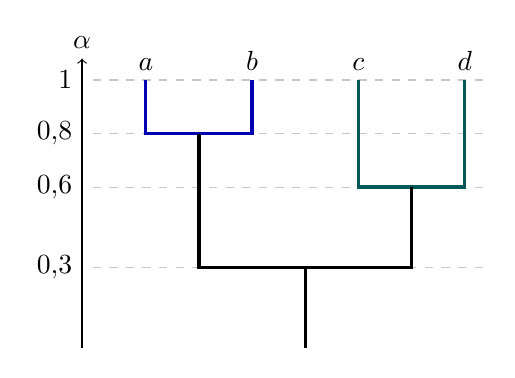
\begin{tikzpicture}[x=1.35cm,y=3.4cm]
\draw[->] (-0.6,0)--(-0.6,1.08) node[above]{$\alpha$};
\foreach \y/\lab in {0.3/{0{,}3},0.6/{0{,}6},0.8/{0{,}8},1/{1}}{
 \draw[gray!45,dashed] (-0.5,\y)--(3.2,\y);
 \node[left] at (-0.6,\y) {$\lab$};
}
\draw[very thick,blue!70!black] (0,1)--(0,0.8)--(1,0.8)--(1,1);
\draw[very thick,teal!70!black] (2,1)--(2,0.6)--(3,0.6)--(3,1);
\draw[very thick] (0.5,0.8)--(0.5,0.3)--(2.5,0.3)--(2.5,0.6);
\draw[very thick] (1.5,0.3)--(1.5,0);
\foreach \x/\lab in {0/a,1/b,2/c,3/d}{\node[above] at (\x,1) {$\lab$};}
\end{tikzpicture}
\end{center}
\end{przyklad}

Nie można zastąpić minimum dowolną normą trójkątną w
Twierdzeniu~\ref{thm:lst-fuzzy-equivalence-cuts}.
Dla $X=\{a,b,c\}$ weźmy relację zwrotną i symetryczną
z $R(a,b)=R(b,c)=1/2$ i $R(a,c)=1/4$.
Jest ona przechodnia względem iloczynu: dla trzech różnych
elementów iloczyn dwóch stopni nie przekracza stopnia
trzeciej pary (wartości to $1/4$ lub $1/8$); gdy elementy
się powtarzają, nierówność wynika z wartości $1$ na przekątnej.
Jednak $E_{1/2}$ nie jest przechodnia.

\subsection{Domknięcie przechodnie}

\begin{twierdzenie}\label{thm:lst-fuzzy-transitive-closure}
Niech $T$ będzie lewostronnie ciągłą normą trójkątną.
Dla relacji rozmytej $R$ na $X$ określmy $R^1=R$,
$R^{n+1}=R\circ_T R^n$. Wówczas
\[
 R^+(x,y)=\sup_{n\geq1}R^n(x,y)
\]
jest najmniejszą $T$-przechodnią relacją rozmytą większą od $R$.
Jeżeli $X$ ma $m\geq1$ elementów, to wystarczy supremum
po $1\leq n\leq m$.
\end{twierdzenie}
\begin{proof}
Zachowywanie supremów przez $T$ oraz łączność składania
dają
\[
 R^+\circ_T R^+=\sup_{i,j\geq1}R^{i+j}\leq R^+,
\]
gdzie suprema relacji są punktowe. Relacja $R^+$ jest
więc przechodnia i zawiera $R$. Jeśli $S\geq R$ jest
$T$-przechodnia, to przez indukcję
$R^{n+1}\leq S\circ_T S\leq S$, zaczynając od $R^1\leq S$.
Stąd $R^+\leq S$.

Dla skończonego $X$, rozwijając definicję składania,
otrzymujemy maksimum iloczynów w sensie $T$ stopni relacji
na ścieżkach długości $n$ od $x$ do $y$.
Jeśli ścieżka ma długość większą niż $m$, to wśród
jej wierzchołków przed wierzchołkiem końcowym występuje
powtórzenie. Usuwamy fragment pomiędzy tymi dwoma
wystąpieniami. Zachowujemy końce i co najmniej jedną
krawędź. Wartość ścieżki nie maleje, gdyż iloczyn w sensie
$T$ usuniętych czynników nie przekracza $1$.
Powtarzając skracanie, otrzymujemy ścieżkę długości
od $1$ do $m$ o wartości nie mniejszej od pierwotnej.
To daje skończony wzór także dla $x=y$.
\end{proof}

\begin{przyklad}[Składanie w skończonym zbiorze]
\label{ex:lst-fuzzy-relation-matrix}
Dla minimum i $X=\{a,b,c\}$ rozważmy macierz
\[
 R=\begin{pmatrix}
 1&0{,}8&0{,}2\\
 0{,}8&1&0{,}6\\
 0{,}2&0{,}6&1
 \end{pmatrix}.
\]
Wpis $(a,c)$ macierzy $R^2$ jest maksimum liczb
$0{,}2,0{,}6,0{,}2$, czyli $0{,}6$.
Pozostałe wpisy poza symetrycznym $(c,a)$ nie zmieniają się:
dla pary $(a,b)$ ścieżka przez $c$ ma wartość $0{,}2$,
a dla $(b,c)$ ścieżka przez $a$ ma wartość $0{,}2$.
Przekątna pozostaje równa $1$. Otrzymana macierz
\[
 R^2=\begin{pmatrix}
 1&0{,}8&0{,}6\\
 0{,}8&1&0{,}6\\
 0{,}6&0{,}6&1
 \end{pmatrix}
\]
jest zwrotna, symetryczna i przechodnia względem minimum:
dla trzech różnych elementów minimum dwóch wpisów
nie przekracza trzeciego, a dla powtórzonych elementów
nierówność wynika z przekątnej. Zatem $R^+=R^2$.
\end{przyklad}

\section{Liczby rozmyte i zasada rozszerzania}
Liczba rozmyta to zbiór rozmyty w $\R$ z górnie półciągłą funkcją
przynależności osiągającą jeden, ograniczonym nośnikiem i przedziałowymi
dodatnimi przekrojami. Te przekroje są niepuste i zwarte.
Dla ciągłej $f:\R^2\to\R$ definiujemy
$\mu_{f(A,B)}(z)=\sup_{f(x,y)=z}\min(\mu_A(x),\mu_B(y))$,
przyjmując $\sup\varnothing=0$ w $[0,1]$.
\begin{twierdzenie}\label{thm:lst-fuzzy-extension-cuts}
Dla liczb rozmytych i $\alpha>0$, $\alpha\leq1$,
$(f(A,B))_\alpha=f(A_\alpha\times B_\alpha)$.
\end{twierdzenie}
\begin{proof}
Inkluzja od prawej do lewej wynika z definicji. Dla punktu
lewej strony wybieramy pary o obrazie $z$ i stopniach większych niż
$\alpha-1/n$ (dla dostatecznie dużych $n$). Dla dużych $n$ należą do zwartego
$A_{\alpha/2}\times B_{\alpha/2}$. Podciąg zbiega do pary
o obrazie $z$ przez ciągłość $f$ i o stopniach co najmniej $\alpha$
przez górną półciągłość funkcji przynależności.
\end{proof}
\begin{wniosek}\label{cor:lst-fuzzy-extension-number}
Dla ciągłej $f:\R^2\to\R$ obraz rozmyty $f(A,B)$
dwóch liczb rozmytych jest liczbą rozmytą.
\end{wniosek}
\begin{proof}
Z Twierdzenia~\ref{thm:lst-fuzzy-extension-cuts} każdy
dodatni przekrój jest ciągłym obrazem niepustego
zwartego spójnego prostokąta. Jest zatem niepustym
zwartym przedziałem. Domkniętość przekrojów daje
górną półciągłość funkcji przynależności, a niepustość
przekroju dla $\alpha=1$ daje osiąganie jedynki.
Jeżeli stopień przynależności obrazu jest dodatni,
istnieje para o dodatnich stopniach przynależności.
Nośnik obrazu zawiera się więc w obrazie przez $f$
iloczynu domknięć nośników $A,B$. Ten iloczyn jest
zwarty, zatem jego obraz jest ograniczony.
\end{proof}

\begin{stwierdzenie}[Arytmetyka przekrojów]\label{prop:lst-fuzzy-interval-arithmetic}
Niech $A_\alpha=[a_-,a_+]$, $B_\alpha=[b_-,b_+]$.
Przy zasadzie rozszerzania z minimum mamy
\[
\begin{split}
 (A+B)_\alpha&=[a_-+b_-,a_++b_+],\\
 (A-B)_\alpha&=[a_--b_+,a_+-b_-],\\
 (AB)_\alpha&=[\min V,\max V],\\
 V&=\{a_-b_-,a_-b_+,a_+b_-,a_+b_+\}.
\end{split}
\]
Jeżeli ponadto $0\notin\overline{\{x:\mu_B(x)>0\}}$,
to iloraz określony zasadą rozszerzania dla $x/y$,
$y\ne0$, jest liczbą rozmytą i
\[
 (A/B)_\alpha=[\min W,\max W],\qquad
 W=\{a_-/b_-,a_-/b_+,a_+/b_-,a_+/b_+\}.
\]
\end{stwierdzenie}
\begin{proof}
Stosujemy Twierdzenie~\ref{thm:lst-fuzzy-extension-cuts}.
Dla sumy i różnicy kresy wyznacza monotoniczność
w poszczególnych argumentach. Dla iloczynu, po ustaleniu
drugiego argumentu, funkcja pierwszego jest afiniczna,
więc kresy występują na końcach pierwszego przedziału.
Po ustaleniu każdego z tych końców stosujemy ten sam
argument do drugiego przedziału. Otrzymujemy cztery
wartości narożne.

W przypadku ilorazu domknięty nośnik $B$ jest zwarty
i oddzielony od zera. W dowodzie zasady rozszerzania
można więc ograniczyć dziedzinę do iloczynu domknięć
nośników, na którym funkcja ilorazu jest ciągła.
Dodatni przekrój $B_\alpha$ jest przedziałem
niezawierającym zera, a jego obraz przez odwrotność
jest przedziałem $[1/b_+,1/b_-]$, ponieważ odwrotność
jest ściśle malejąca na każdej półosi.
Wzór dla iloczynu daje cztery wartości ilorazowe.
Argument z Wniosku~\ref{cor:lst-fuzzy-extension-number}
działa również tutaj, z ograniczoną dziedziną funkcji.
\end{proof}

\begin{przyklad}[Dodawanie i odejmowanie liczb trójkątnych]
\label{ex:lst-fuzzy-triangular-arithmetic}
Dla liczb trójkątnych $A=(1,2,4)$, $B=(0,3,5)$
mamy $A_\alpha=[1+\alpha,4-2\alpha]$ i
$B_\alpha=[3\alpha,5-2\alpha]$.
Wynika stąd
\[
 (A+B)_\alpha=[1+4\alpha,9-4\alpha],
 \qquad
 (A-B)_\alpha=[-4+3\alpha,4-5\alpha].
\]
Z rekonstrukcji przekrojów otrzymujemy liczby trójkątne
$A+B=(1,5,9)$ i $A-B=(-4,-1,4)$.
\begin{center}
\begin{tikzpicture}[x=0.53cm,y=2.7cm,>=Stealth]
\draw[->] (-4.6,0)--(10,0) node[right]{$x$};
\draw[->] (0,0)--(0,1.16) node[above]{$\mu$};
\draw[gray!65,dashed] (-4.2,0.5)--(9.2,0.5);
\draw[thick,blue!75!black] (1,0)--(2,1)--(4,0);
\draw[thick,teal!75!black] (0,0)--(3,1)--(5,0);
\draw[very thick,orange!85!black] (1,0)--(5,1)--(9,0);
\draw[very thick,violet!80!black] (-4,0)--(-1,1)--(4,0);
\node[above,blue!75!black] at (2,1) {$A$};
\node[above,teal!75!black] at (3,1) {$B$};
\node[above,orange!85!black] at (5,1) {$A+B$};
\node[above,violet!80!black] at (-1,1) {$A-B$};
\foreach \x in {-4,-1,1,4,5,9}{\node[below] at (\x,0) {$\x$};}
\node[below left] at (0,0) {$0$};
\end{tikzpicture}
\end{center}
\end{przyklad}

\begin{uwaga}[Zależność argumentów]\label{rem:lst-fuzzy-dependent-arguments}
Zasada rozszerzania dla dwóch niezależnie wybieranych
argumentów nie zachowuje ich utożsamienia.
Jeżeli $A=(1,2,4)$, to z powyższych wzorów
$(A-A)_\alpha=[-3+3\alpha,3-3\alpha]$.
Nie jest to ostra liczba $0$. Natomiast obraz jednej
zmiennej przez funkcję $x\mapsto x-x=0$ jest ostrą
liczbą $0$: jej stopień w zerze wynosi $1$, a w każdym
innym punkcie $0$. Różnica pochodzi z dopuszczenia
dwóch różnych realizacji tej samej liczby rozmytej.
\end{uwaga}



\section{Wnioskowanie rozmyte}
Stopnie przynależności mogą opisywać pojęcia takie jak
niska lub wysoka temperatura. Reguła łączy rozmyte
przesłanki z rozmytym albo liczbowym wnioskiem.
Nie należy jednak utożsamiać inżynierskich metod
wnioskowania rozmytego z rachunkiem dowodów MTL:
operacje agregacji i defuzyfikacji stanowią dodatkowe
elementy modelu.

\subsection{Metoda Mamdaniego}
\begin{definicja}\label{def:lst-fuzzy-mamdani}
Dla danych wejściowych $x=(x_1,\ldots,x_n)$ rozważmy
$m$ reguł postaci
\[
 \text{jeżeli }x_1\text{ jest }A_{i1},\ldots,
 x_n\text{ jest }A_{in},\text{ to }y\text{ jest }B_i.
\]
W wersji minimum--maksimum stopień aktywacji $w_i$,
obcięta funkcja wyjściowa i agregacja mają postać
\[
\begin{split}
 w_i&=\min_{1\leq j\leq n}\mu_{A_{ij}}(x_j),\\
 \nu_i(y)&=\min(w_i,\mu_{B_i}(y)),\\
 \nu(y)&=\max_{1\leq i\leq m}\nu_i(y).
\end{split}
\]
Jeżeli $\nu$ jest mierzalna,
$0<\int_\R\nu\,\mathrm d\lambda_1<\infty$ i
$\int_\R |y|\nu(y)\,\mathrm d\lambda_1(y)<\infty$, to
defuzyfikacja metodą środka ciężkości daje
\[
 y_*=\frac{\int_\R y\nu(y)\,\mathrm d\lambda_1(y)}
 {\int_\R\nu(y)\,\mathrm d\lambda_1(y)}.
\]
\end{definicja}
Jeżeli wszystkie reguły mają zerową aktywację, mianownik
jest zerem i metoda środka ciężkości nie wyznacza wyniku.
Potrzebna jest wówczas osobna reguła postępowania.
Wzór używa całek względem miary Lebesgue'a, a nie stopni
prawdopodobieństwa: normalizacja pozwala traktować
$\nu/\int_\R\nu\,\mathrm d\lambda_1$ jako gęstość,
lecz nie jest to interpretacja pierwotnych stopni prawdy.

\begin{przyklad}[Pełne obliczenie metodą Mamdaniego]
\label{ex:lst-fuzzy-mamdani-centroid}
Niech $x\in[0,1]$ będzie znormalizowanym wejściem.
Przyjmijmy funkcje przesłanek $\mu_{A_1}(x)=1-x$
i $\mu_{A_2}(x)=x$. Dla $x=3/4$ aktywacje wynoszą
$w_1=1/4$, $w_2=3/4$.
Wnioski są trójkątnymi liczbami rozmytymi
$B_1=(0,2,4)$ i $B_2=(4,6,8)$.
Zatem obie funkcje wyjściowe mają rozłączne dodatnie
nośniki; stykają się tylko w punkcie $4$, gdzie obie
są równe zero. Agregacja maksimum jest w tym przykładzie
równa ich sumie.

Dla trójkąta o środku $c$, połowie szerokości $h>0$
i wysokości $1$ funkcja przynależności ma postać
$\mu(y)=\max(0,1-|y-c|/h)$.
Po obcięciu na wysokości $w\in[0,1]$ otrzymujemy
$\nu_w(y)=\min(w,\mu(y))$. Symetria względem $c$
oraz podstawienie $t=|y-c|$ dają
\[
\begin{split}
 I(w)&=\int_\R\nu_w(y)\,\mathrm d\lambda_1(y)\\
 &=2\left(\int_0^{h(1-w)}w\,\mathrm d\lambda_1(t)
 +\int_{h(1-w)}^h(1-t/h)\,\mathrm d\lambda_1(t)\right)\\
 &=2h w-hw^2,\\
 \int_\R y\nu_w(y)\,\mathrm d\lambda_1(y)&=cI(w).
\end{split}
\]
W ostatnim wzorze całka z $(y-c)\nu_w(y)$ jest zerem
przez symetrię. Dla $h=2$ otrzymujemy
$I(1/4)=7/8$ i $I(3/4)=15/8$. W konsekwencji
\[
 y_*=\frac{2\cdot7/8+6\cdot15/8}{7/8+15/8}
 =\frac{52}{11}\approx4{,}727.
\]
\begin{center}
\begin{tikzpicture}[x=0.9cm,y=3cm,>=Stealth]
\fill[blue!16] (0,0)--(0.5,0.25)--(3.5,0.25)--(4,0)--cycle;
\fill[teal!22] (4,0)--(5.5,0.75)--(6.5,0.75)--(8,0)--cycle;
\draw[gray,dashed] (0,0)--(2,1)--(4,0)--(6,1)--(8,0);
\draw[very thick,blue!75!black] (0,0)--(0.5,0.25)--(3.5,0.25)--(4,0);
\draw[very thick,teal!75!black] (4,0)--(5.5,0.75)--(6.5,0.75)--(8,0);
\draw[->] (-0.2,0)--(8.5,0) node[right]{$y$};
\draw[->] (0,0)--(0,1.15) node[above]{$\nu(y)$};
\draw[orange!85!black,thick,dashed] ({52/11},0)--({52/11},0.95);
\node[above,orange!85!black] at ({52/11},0.95) {$y_*$};
\foreach \x in {0,2,4,6,8}{\node[below] at (\x,0) {$\x$};}
\node[left] at (0,0.25) {$1/4$};
\node[left] at (0,0.75) {$3/4$};
\end{tikzpicture}
\end{center}
Rysunek przedstawia funkcje przed obcięciem (linie
przerywane), agregację (wypełnienie) i wynik defuzyfikacji.
Jeżeli nośniki wniosków zachodzą na siebie, nie wolno
zastąpić agregacji maksimum ich sumą, ponieważ
wspólny obszar zostałby policzony dwukrotnie.
\end{przyklad}

\subsection{Metoda Takagiego--Sugeno}
\begin{definicja}\label{def:lst-fuzzy-sugeno}
W metodzie Takagiego--Sugeno wniosek $i$-tej reguły
jest funkcją liczbową $f_i(x)$, a nie zbiorem rozmytym.
Dla nieujemnych aktywacji $w_i(x)$ o dodatniej sumie
wyjście jest określone przez
\[
 y_{\mathrm S}(x)=
 \frac{\sum_{i=1}^m w_i(x)f_i(x)}{\sum_{i=1}^m w_i(x)}.
\]
W systemie zerowego rzędu $f_i$ są stałe,
a w systemie pierwszego rzędu są funkcjami afinicznymi.
\end{definicja}
Po normalizacji współczynniki
$\theta_i=w_i/\sum_jw_j$ są nieujemne i sumują się do $1$.
Wyjście jest więc kombinacją wypukłą wartości $f_i(x)$:
\[
 \min_i f_i(x)\leq y_{\mathrm S}(x)\leq\max_i f_i(x).
\]
Obie nierówności otrzymujemy, mnożąc odpowiednie
ograniczenie każdego $f_i(x)$ przez $\theta_i$ i sumując.

\begin{przyklad}[Porównanie metod]\label{ex:lst-fuzzy-sugeno-comparison}
Dla tych samych aktywacji co w
Przykładzie~\ref{ex:lst-fuzzy-mamdani-centroid}
i stałych konsekwencji $f_1=2$, $f_2=6$ otrzymujemy
$y_{\mathrm S}=2/4+18/4=5$.
Nie jest to wynik Mamdaniego $52/11$.
Metoda Sugeno waży środki bezpośrednio aktywacjami,
natomiast w przykładzie Mamdaniego wagi są polami
obciętych trójkątów, proporcjonalnymi do $2w-w^2$.
Dla $x\in[0,1]$ w rozważanym systemie Sugeno mamy
$w_1=1-x$, $w_2=x$, a zatem $y_{\mathrm S}(x)=2+4x$.
W metodzie Mamdaniego dla tych samych wejść i trójkątów
\[
 y_{\mathrm M}(x)=
 \frac{2(1-x^2)+6(2x-x^2)}{1+2x-2x^2}.
\]
Wzór otrzymujemy przez podstawienie $w_1=1-x$, $w_2=x$
do $I(w)=4w-2w^2$ i skrócenie czynnika $2$.
Mianownik jest dodatni na całym $[0,1]$.
\begin{center}
\begin{tikzpicture}[x=6cm,y=0.65cm,>=Stealth]
\draw[->] (0,0)--(1.12,0) node[right]{$x$};
\draw[->] (0,0)--(0,6.7) node[above]{$y$};
\foreach \y in {2,4,6}{\draw[gray!40,dashed] (0,\y)--(1,\y);
 \node[left] at (0,\y) {$\y$};}
\draw[blue!75!black,very thick,domain=0:1,samples=60]
 plot (\x,{2+4*\x});
\draw[orange!85!black,very thick,domain=0:1,samples=60]
 plot (\x,{(2*(1-\x*\x)+6*(2*\x-\x*\x))/(1+2*\x-2*\x*\x)});
\draw[gray,dashed] (0.75,0)--(0.75,5);
\foreach \x/\lab in {0/0,0.5/{1/2},0.75/{3/4},1/1}
 {\node[below] at (\x,0) {$\lab$};}
\node[blue!75!black,anchor=west] at (0.13,5.9) {Sugeno};
\node[orange!85!black,anchor=west] at (0.13,5.2) {Mamdani};
\end{tikzpicture}
\end{center}
\end{przyklad}

\begin{uwaga}
W obu metodach funkcje przynależności, wybór normy,
baza reguł i sposób agregacji wymagają uzasadnienia
w konkretnym modelu. Rachunek logiczny nie wyznacza
automatycznie tych danych. Wynik defuzyfikacji jest
pojedynczą liczbą, nie stopniem prawdziwości wniosku.
\end{uwaga}
